% =============================================================
% Lab 1 - Informe HTTP / DNS (formato IEEE)
% Cada pregunta incluye un placeholder de figura con un nombre
% descriptivo. Cambia el nombre del archivo de imagen dentro de
% \includegraphics{} según corresponda a tu evidencia.
% =============================================================
 

\subsection{Checkpoint 1: Simple UDP Capture}
\begin{enumerate}

\item \textbf{How many UDP packets were captured during your session? Were they mostly sent or received by your host?}

En la captura filtrada se observan 19 paquetes UDP asociados con nuestro equipo, \texttt{172.20.10.7}: 9 enviados y 10 recibidos (Fig.~\ref{fig:chk1-1}). Por tanto, se recibieron ligeramente más paquetes de los que se enviaron. Al filtrar la dirección 34.139.173.2, asociada con la página de UTEC en esta prueba, el tráfico mostrado corresponde a TCP y TLS, no a UDP  (Fig.~\ref{fig:chk1-2}).

\begin{figure}[htbp]
    \centering
    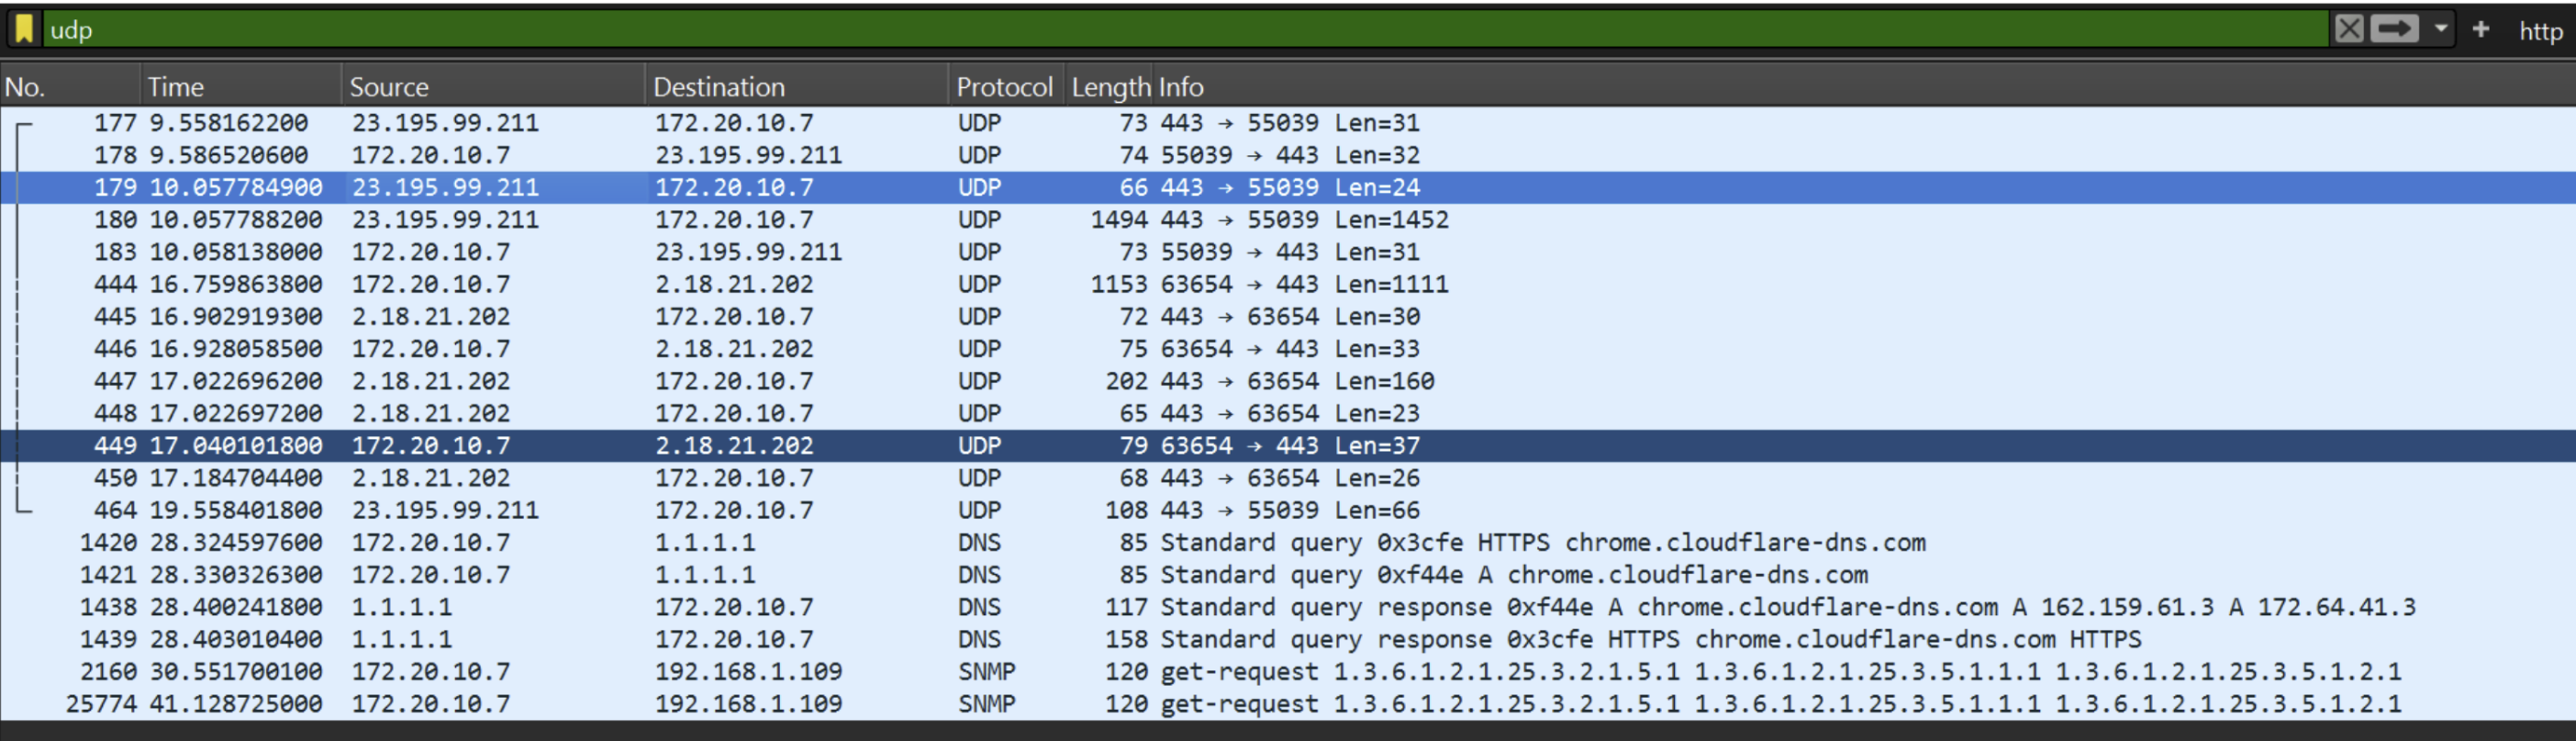
\includegraphics[width=1\linewidth]{imgs/check1_1.png}
    \caption{Paquetes UDP enviados y recibidos durante la captura.}
    \label{fig:chk1-1}
\end{figure}
 
\begin{figure}[htbp]
    \centering
    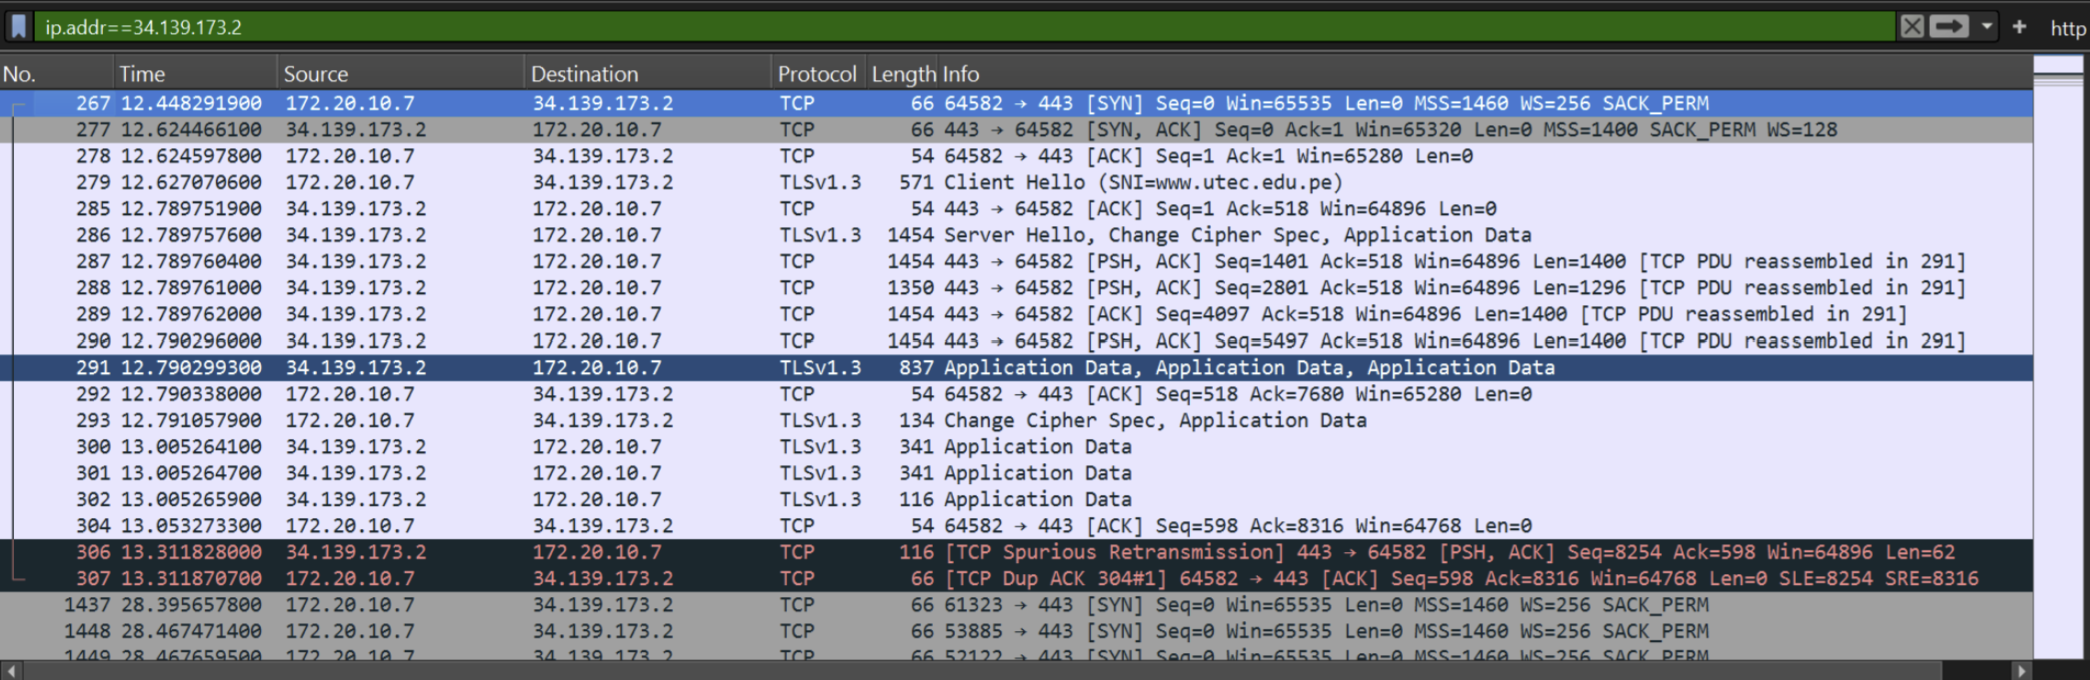
\includegraphics[width=1\linewidth]{imgs/check1_2.png}
    \caption{Tráfico TCP y TLS registrado hacia la dirección IP de UTEC.}
    \label{fig:chk1-2}
\end{figure}

\item \textbf{Did you notice any UDP traffic that was not related to accessing the www.utec.edu.pe website? If so, what could be the source of that traffic?}

Sí, durante la sesión si hubo tráfico UDP que no estaba relacionado al acceso a www.utec.edu.pe (Fig.~\ref{fig:chk1-3}). Las consultas DNS podrían proceder del navegador o de procesos en segundo plano.

\begin{figure}[htbp]
    \centering
    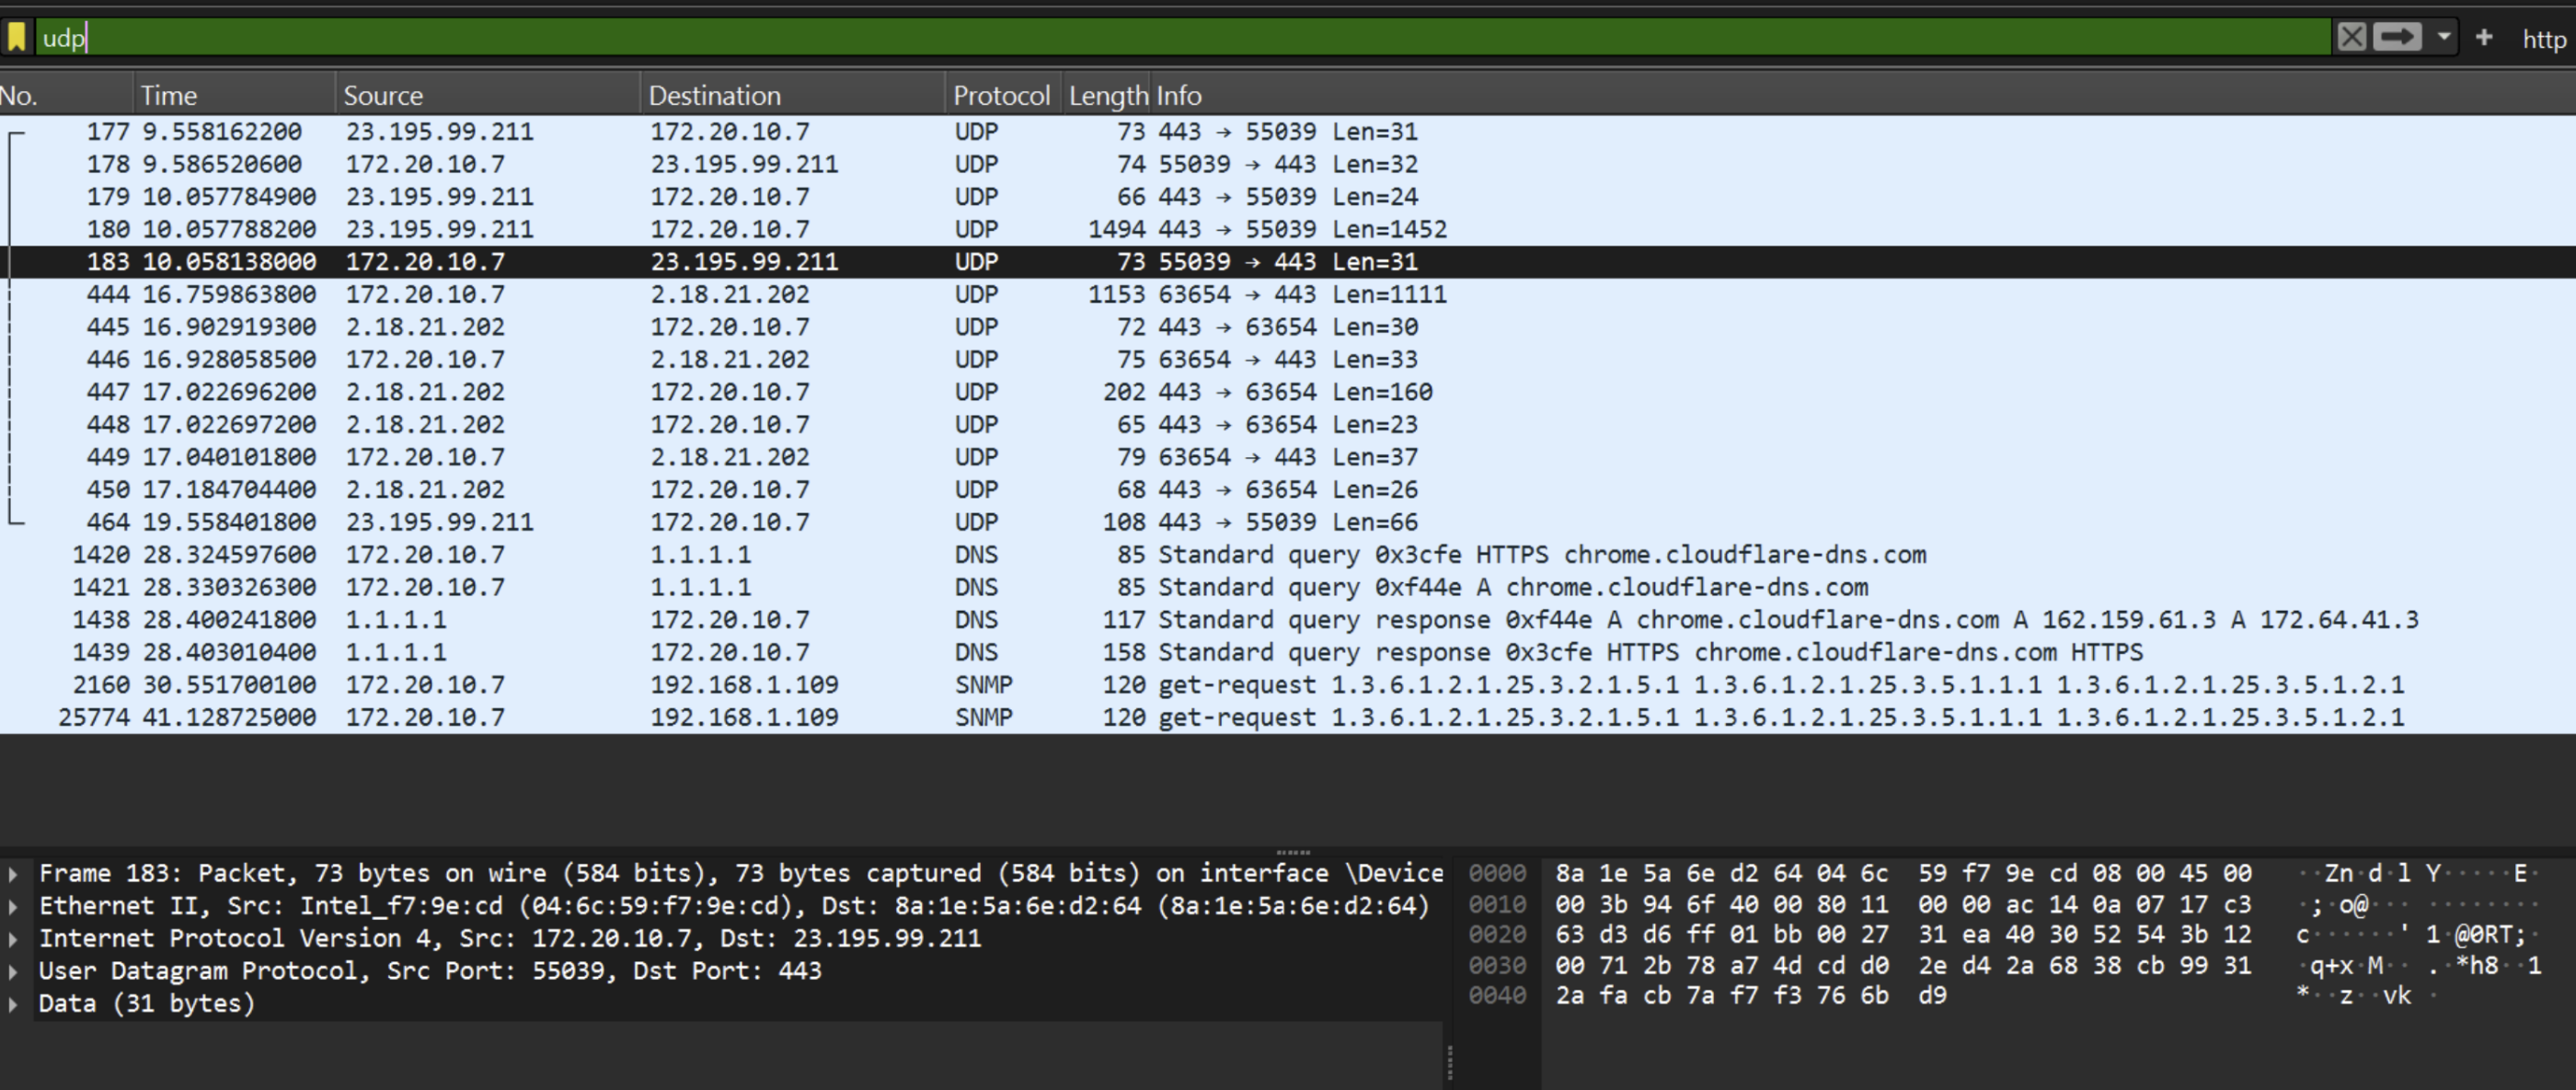
\includegraphics[width=1\linewidth]{imgs/check1_3.png}
    \caption{Paquetes UDP con destinos distintos a la página de UTEC.}
    \label{fig:chk1-3}
\end{figure}

\item \textbf{Pick a UDP packet from your host and describe its main fields (e.g., source port, destination port, length, checksum).}

\begin{figure}[htbp]
    \centering
    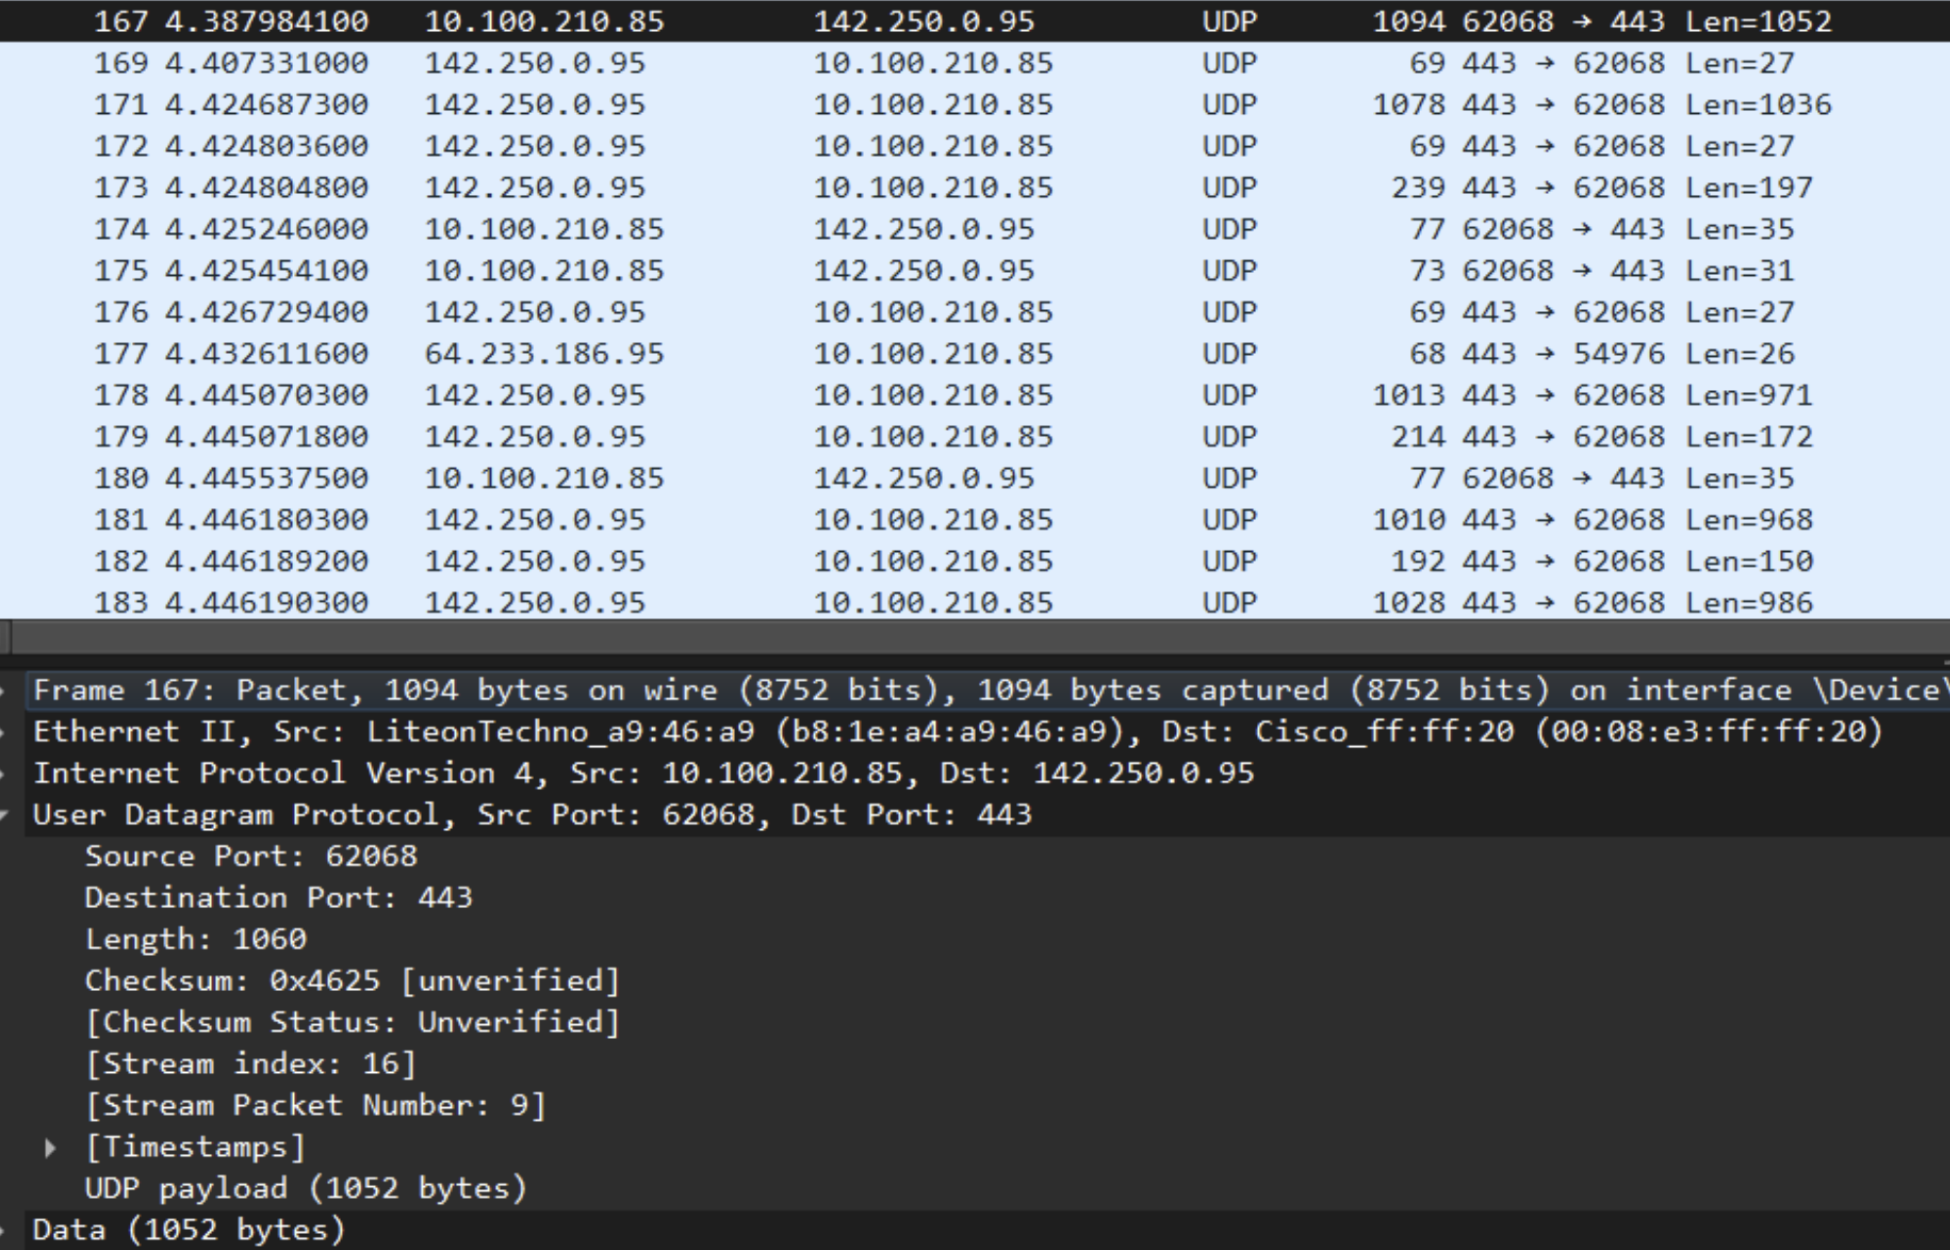
\includegraphics[width=1\linewidth]{imgs/check1_4.png}
    \caption{Puertos, longitud y checksum del datagrama UDP seleccionado.}
    \label{fig:chk1-4}
\end{figure}

Campos principales de un paquete UDP (Fig.~\ref{fig:chk1-4}) : 
\begin{itemize}
    \item Source port: 62068
    \item Destination port: 443
    \item Length: 1060 bytes
    \item Checksum: 0x4625 [unverified]
\end{itemize}


\item \textbf{Is the UDP checksum marked as verified or unverified? What does this indicate in the context of your operating system and network interface?}

Está marcado como unverified (Fig.~\ref{fig:chk1-4}). Unverified checksum indica que el cálculo del checksum no fue verificado por Wireshark, esto posiblemente se da porque el cálculo fue delegado a la tarjeta de red. 

\item \textbf{Compare UDP with TCP based on what you observed in Wireshark. What are the key differences in terms of packet structure and reliability?}

En la captura de Wireshark realizada, se puede comprobar la alta confiabilidad de TCP a través de sus banderas. Observamos paquetes con la etiqueta [ACK] lo que demuestra el mecanismo de reporte de saludo que utiliza TCP para confirmar que los datos llegaron a su destino. También se aprecian banderas [PSH] , utilizadas para forzar la entrega inmediata de datos a la aplicación (Fig.~\ref{fig:chk1-6}). En contraste, los paquetes UDP no poseen estas banderas de control ni realizan confirmaciones, enviando los datos sin garantizar su recepción (Fig.~\ref{fig:chk1-5}). 

\begin{figure}[htbp]
    \centering
    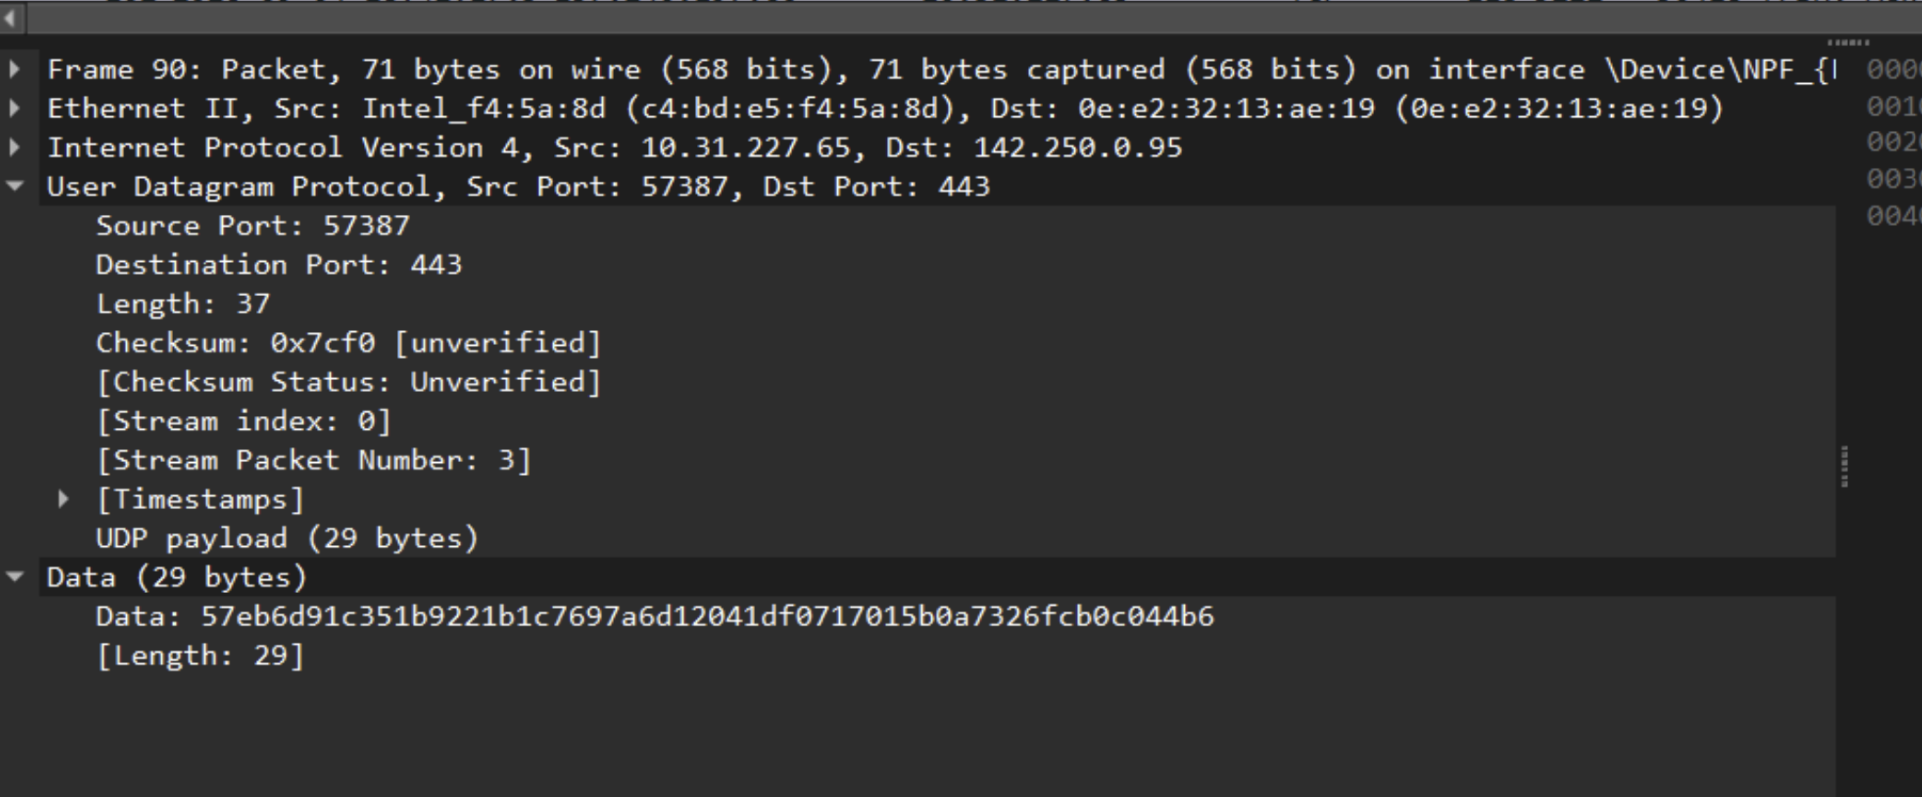
\includegraphics[width=1\linewidth]{imgs/check1_5.png}
    \caption{Campos del datagrama UDP utilizado para la comparación.}
    \label{fig:chk1-5}
\end{figure}

\begin{figure}[htbp]
    \centering
    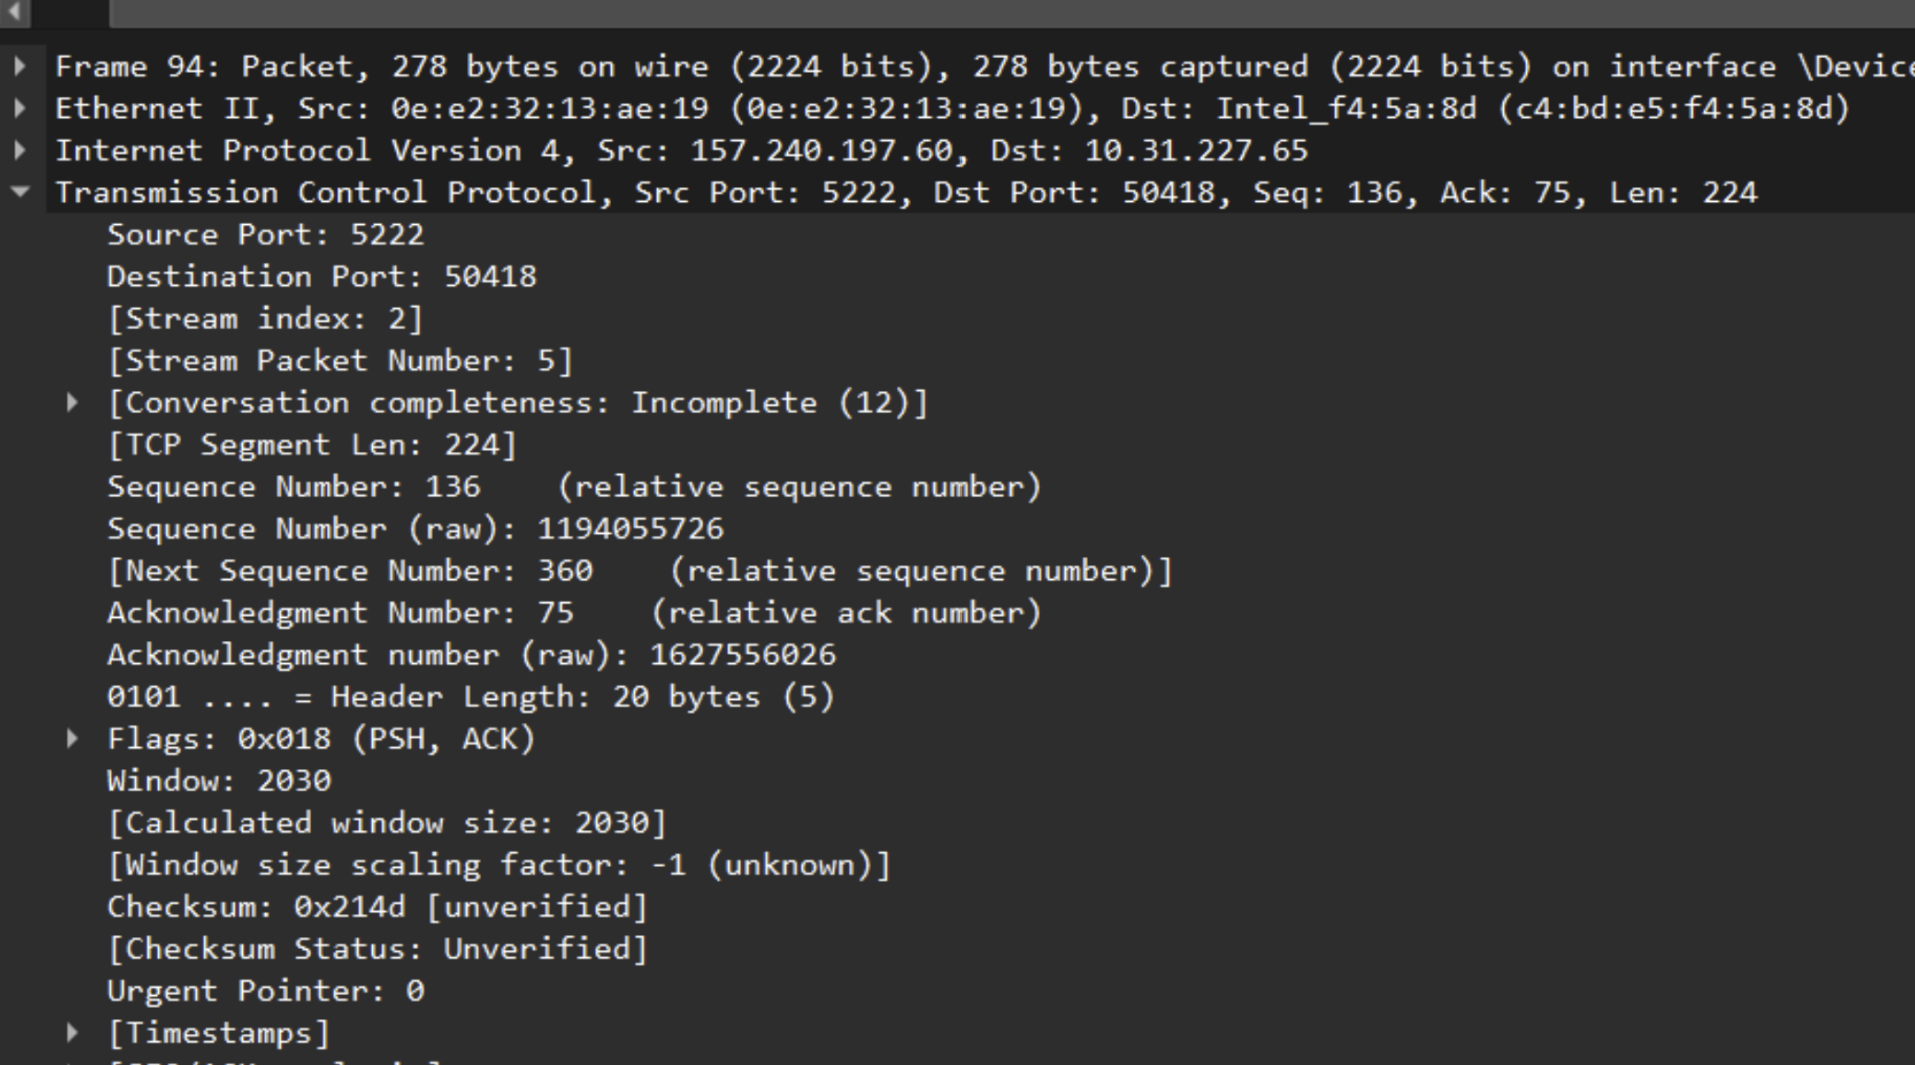
\includegraphics[width=1\linewidth]{imgs/check1_6.png}
    \caption{Campos y banderas del segmento TCP utilizado para la comparación.}
    \label{fig:chk1-6}
\end{figure}

\item \textbf{What are the potential risks or vulnerabilities of using UDP in a network? Did you observe any unusual or potentially malicious UDP traffic?}

Como UDP no confirma ni retransmite los datagramas, algunos riesgos o vulnerabilidades de usar UDP en un network es que los paquetes enviados se pueden perderse, duplicarse o llegar desordenados. Así mismo, este facilita la falsificación de direcciones IP y ataques DDos donde pueden saturar un servidor o red \cite{rfc768,gelenbe2023flood}. Durante la captura no se observó tráfico UDP inusual o potencialmente malicioso. Los paquetes que se registraron parecen ser de servicios normales ejecutados en segundo plano por el navegador o el sistema (Fig.~\ref{fig:chk1-1}).

\item \textbf{How could an administrator use Wireshark to detect suspicious UDP behavior, such as a port scan or DDoS attempt?}

Un administrador puede utilizar Wireshark para monitorear el tráfico UDP y detectar anomalías analizando los siguientes indicadores \cite{wireshark_guide}:

\begin{itemize}
\item \textbf{Detección de Port Scanning:} Al aplicar un filtro de tráfico UDP y revisar el panel Statistics > Conversations, el administrador puede identificar si una misma dirección IP de origen intenta establecer comunicación con múltiples puertos de un host destino en un lapso corto de tiempo. Un patrón recurrente de mensajes ICMP \textit{Destination Unreachable (Port Unreachable)} devueltos también suele ser indicativo de un escaneo activo.
\item \textbf{Detección de DDoS:} Utilizando Statistics > I/O Graphs, se puede visualizar un aumento abrupto en la densidad de paquetes por segundo (pks/sec) hacia un equipo o red específica. Al cruzar este pico con el panel de conversaciones, se observará un tráfico masivo desde una o múltiples fuentes que contrasta drásticamente con la línea base de uso habitual.
\end{itemize}

\end{enumerate}





 \subsection{Checkpoint 2: Using nslookup}
\begin{enumerate}

\item \textbf{How many UDP packets were captured during the nslookup www.cisco.com query? Were they sent, received, or both?}

En la lista se observan cuatro paquetes DNS asociados con
las consultas de www.cisco.com: dos solicitudes
enviadas por el equipo y dos respuestas recibidas
(Fig.~\ref{fig:chk2-1} y Fig.~\ref{fig:chk2-2}).

\begin{figure}[htbp]
    \centering
    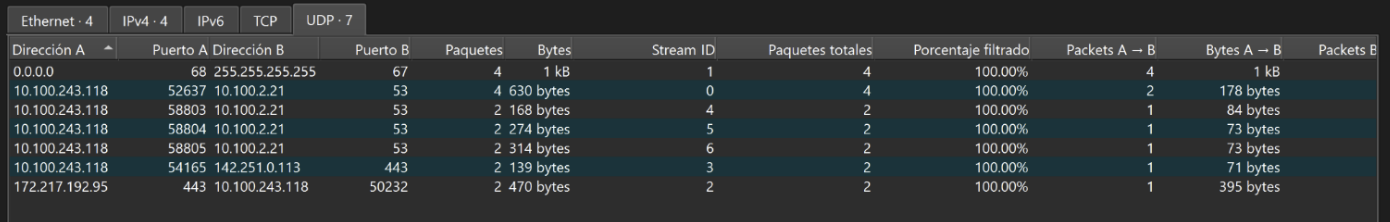
\includegraphics[width=1\linewidth]{imgs/check2_1.png}
    \caption{Conversaciones UDP registradas durante la consulta DNS.}
    \label{fig:chk2-1}
\end{figure}

\begin{figure}[htbp]
    \centering
    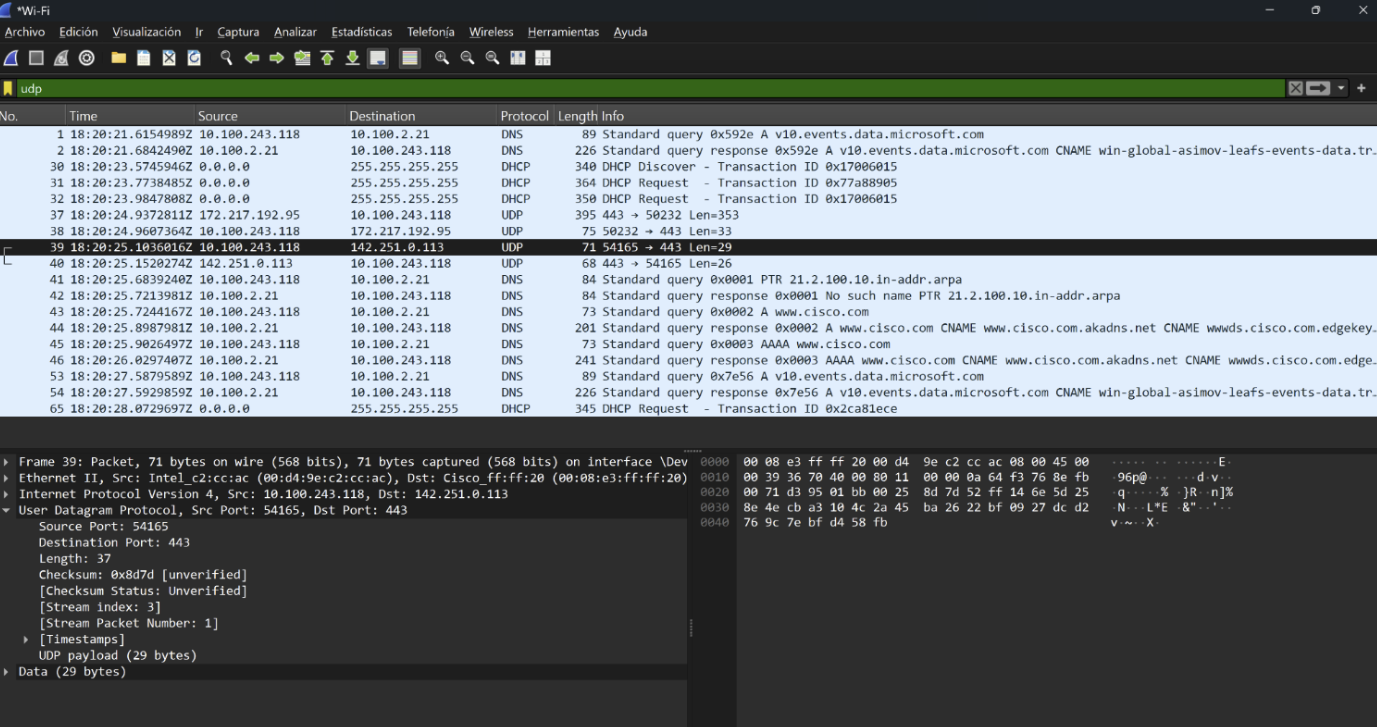
\includegraphics[width=1\linewidth]{imgs/check2_2.png}
    \caption{Solicitudes y respuestas DNS observadas en Wireshark.}
    \label{fig:chk2-2}
\end{figure}

\item \textbf{What are the source and destination port numbers of the captured DNS packets? What does this indicate about how DNS communication works?}

En una de las solicitudes se observa el puerto de origen 58803 y el puerto de destino 53 (Fig.~\ref{fig:chk2-6}). El equipo utiliza un puerto temporal y dirige la consulta al puerto DNS del servidor. En la respuesta correspondiente, el servidor utiliza el puerto 53 como origen y responde al puerto temporal de esa solicitud \cite{rfc1035}.




\item \textbf{Describe the typical UDP length for the DNS request and response observed. Are the packet sizes similar or different? Why might that be?}

Una de las solicitudes tiene una longitud UDP de 73 bytes, y las respuestas son mayores, de 201 y 241 bytes (Fig.~\ref{fig:chk2-6}). Las respuestas son más largas porque tienen información adicional como direcciones IP y records CNAME.


\item \textbf{Was the DNS query resolved successfully? How can you tell this by analyzing the UDP response in Wireshark?}

Sí, la DNS query respondio correctamente. Lo podemos identificar ya que la respuesta seleccionada tuvo en su flags tiene la etiqueta \textit{Standard query response, No error} y tiene registros normales de respuesta (Fig.~\ref{fig:chk2-3}).

\begin{figure}[htbp]
    \centering
    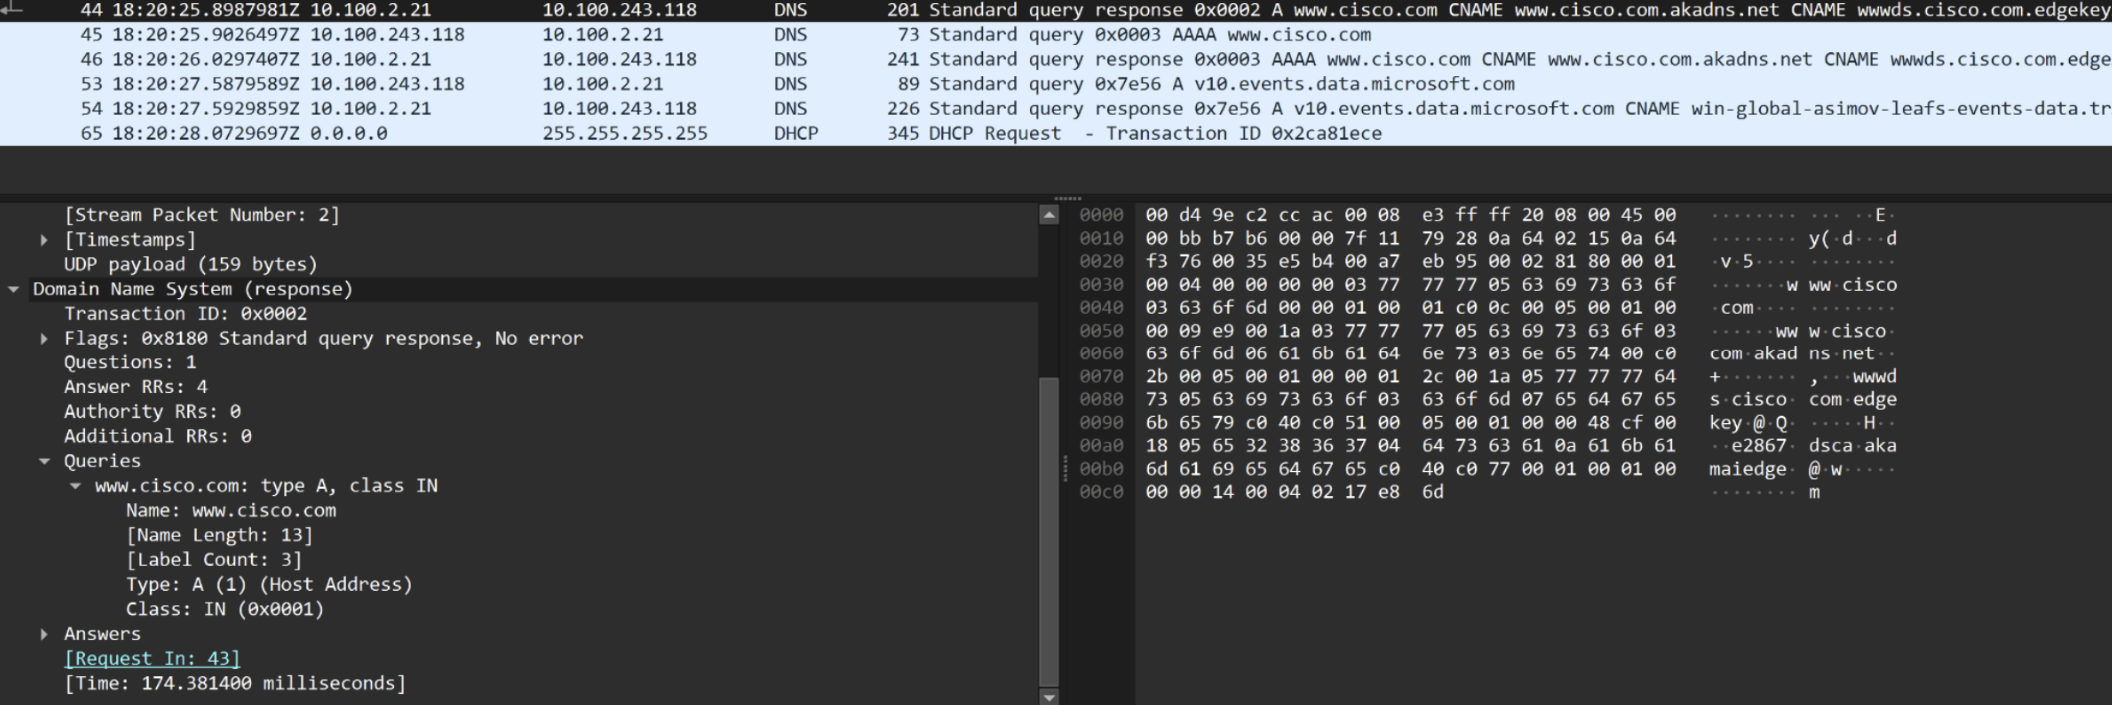
\includegraphics[width=1\linewidth]{imgs/check2_3.png}
    \caption{Respuesta DNS de www.cisco.com sin errores y con registros en Answers.}
    \label{fig:chk2-3}
\end{figure}


\item \textbf{Why is DNS usually implemented over UDP instead of TCP? Based on your observations, what advantages does UDP offer in this case?}

Los DNS usualmente utilizan UDP en vez de TCP porque UDP permite enviar una consulta DNS y recibir su respuesta
sin establecer antes una conexión TCP. Esto evita el
intercambio inicial necesario para abrir esa conexión y
resulta una ventaja al ser más práctico para consultas cortas. 

\item \textbf{Expand the UDP layer of a selected DNS packet. What are the values of the source port, destination port, length, and checksum? Provide a brief explanation of each field}

En el paquete seleccionado, el Source Port es
53, el Destination Port es 58804, Length es de 167 bytes y el Checksum es 0xeb95 (Fig.~\ref{fig:chk2-4}). El source y destination port identifican el envio y el recibo; el length especifica el tamaño del UDP header y payload, y el checksum se usa para detectar errores en el datagrama \cite{rfc768}. 

\begin{figure}[htbp]
    \centering
    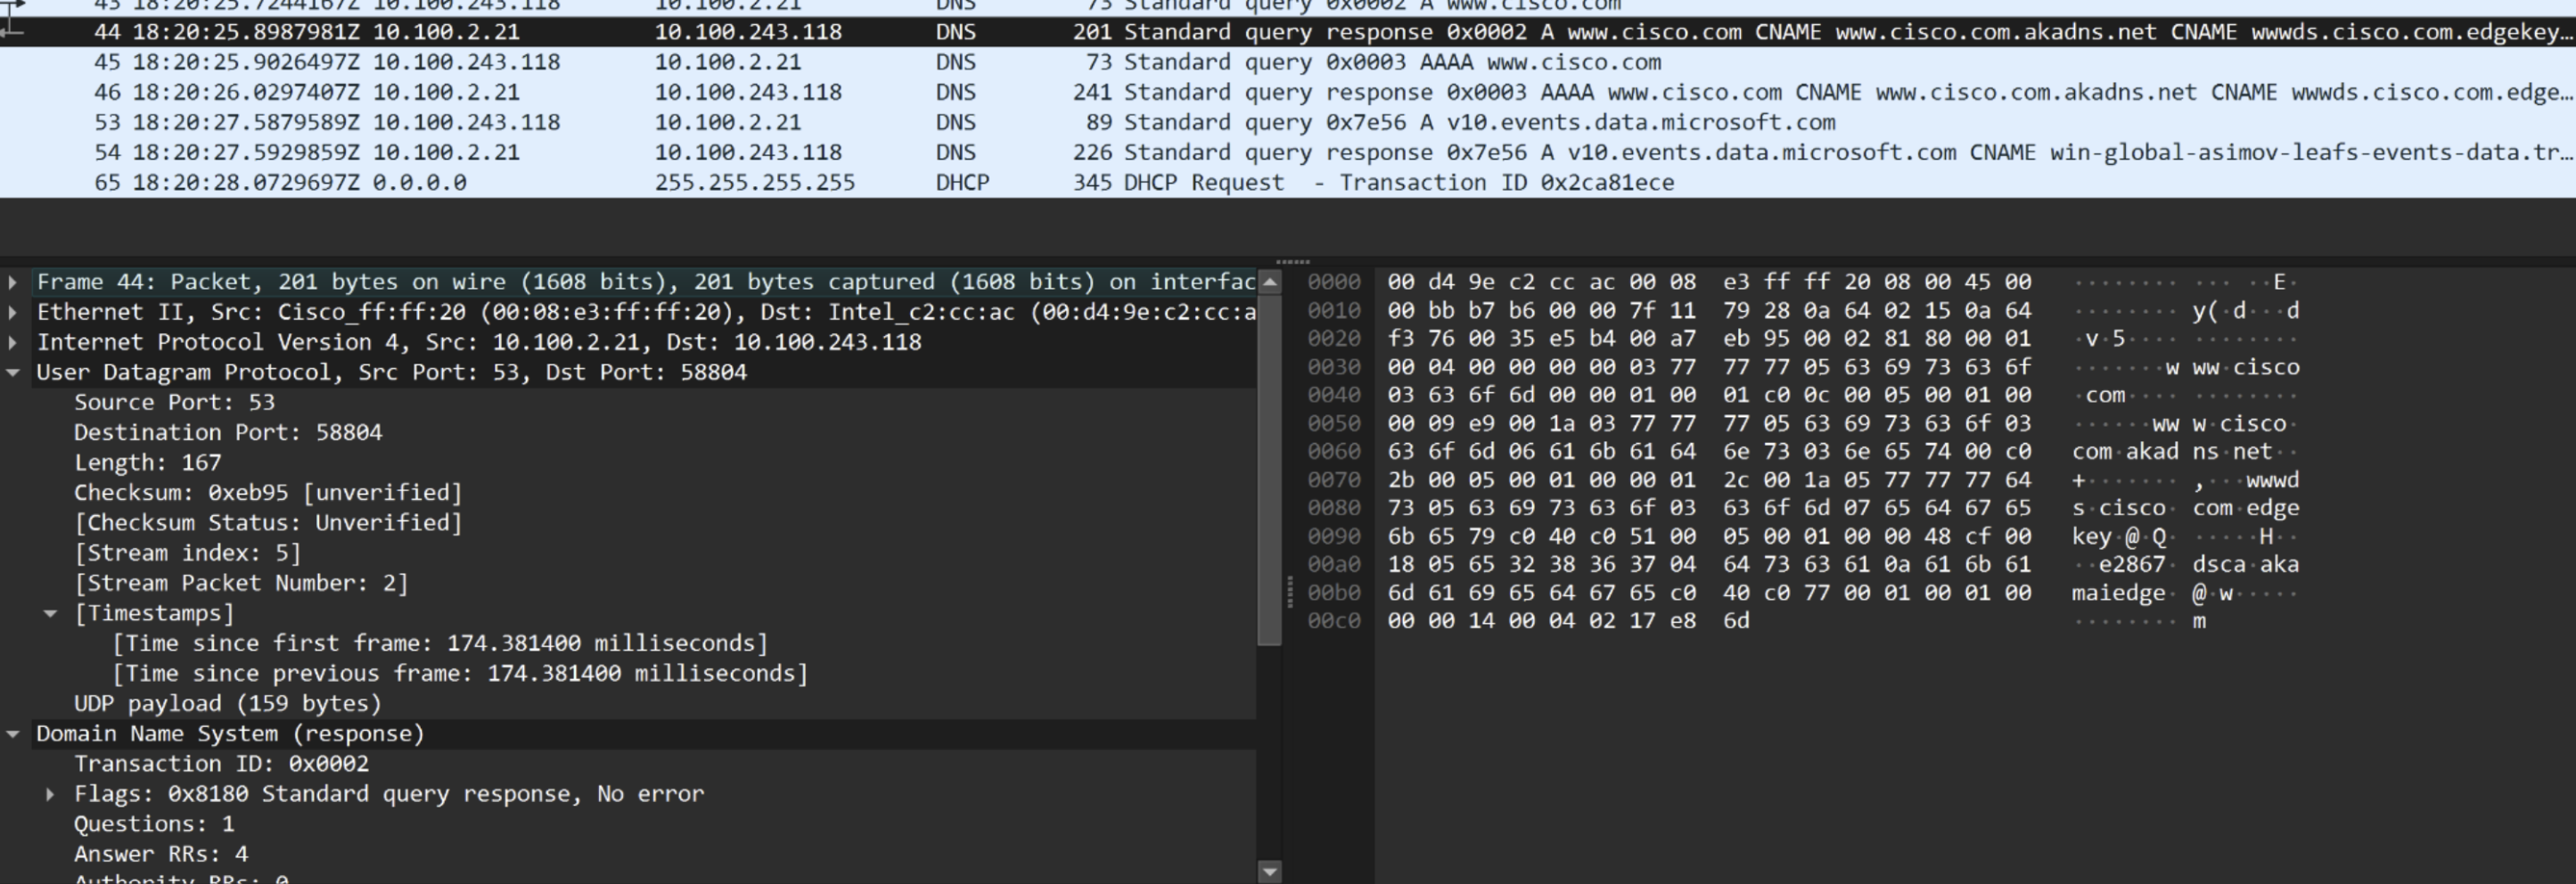
\includegraphics[width=1\linewidth]{imgs/check2_4.png}
    \caption{Puertos, longitud y checksum de una respuesta DNS transportada por UDP.}
    \label{fig:chk2-4}
\end{figure}

\item \textbf{What is the maximum number of bytes that can be included in a UDP payload? (Research and present in the lab session)}

En IPv4, con un encabezado IP mínimo de 20 bytes, el máximo teórico de datos de un datagrama UDP es de 65\,507 bytes. Se obtiene al restar al máximo de 65\,535 bytes del paquete IPv4 los 20 bytes de su encabezado y los 8 bytes del encabezado UDP: \(65\,535-20-8=65\,507\) \cite{rfc768,kurose2021}. Ese máximo teórico no garantiza que un datagrama de ese tamaño pueda enviarse o recibirse completo por cualquier trayecto \cite{rfc8900}.


\item \textbf{What is the largest possible source port number? (Research and present in
the lab session).}

Los puertos usan 16 bits, por lo que el mayor número que puede representar el campo de puerto de origen es \(2^{16}-1=65\,535\) \cite{rfc768}.

\item \textbf{What is the protocol number for UDP? Give your answer in both hexadecimal and decimal notation. To answer this question, you’ll need to look into the Protocol field of the IP datagram containing this UDP segment.}

En el campo Protocol del encabezado IP se observa el valor 17 en decimal, equivalente a 0x11 en hexadecimal (Fig.~\ref{fig:chk2-5}). Este valor identifica a UDP como el protocolo transportado por IP.

\begin{figure}[htbp]
    \centering
    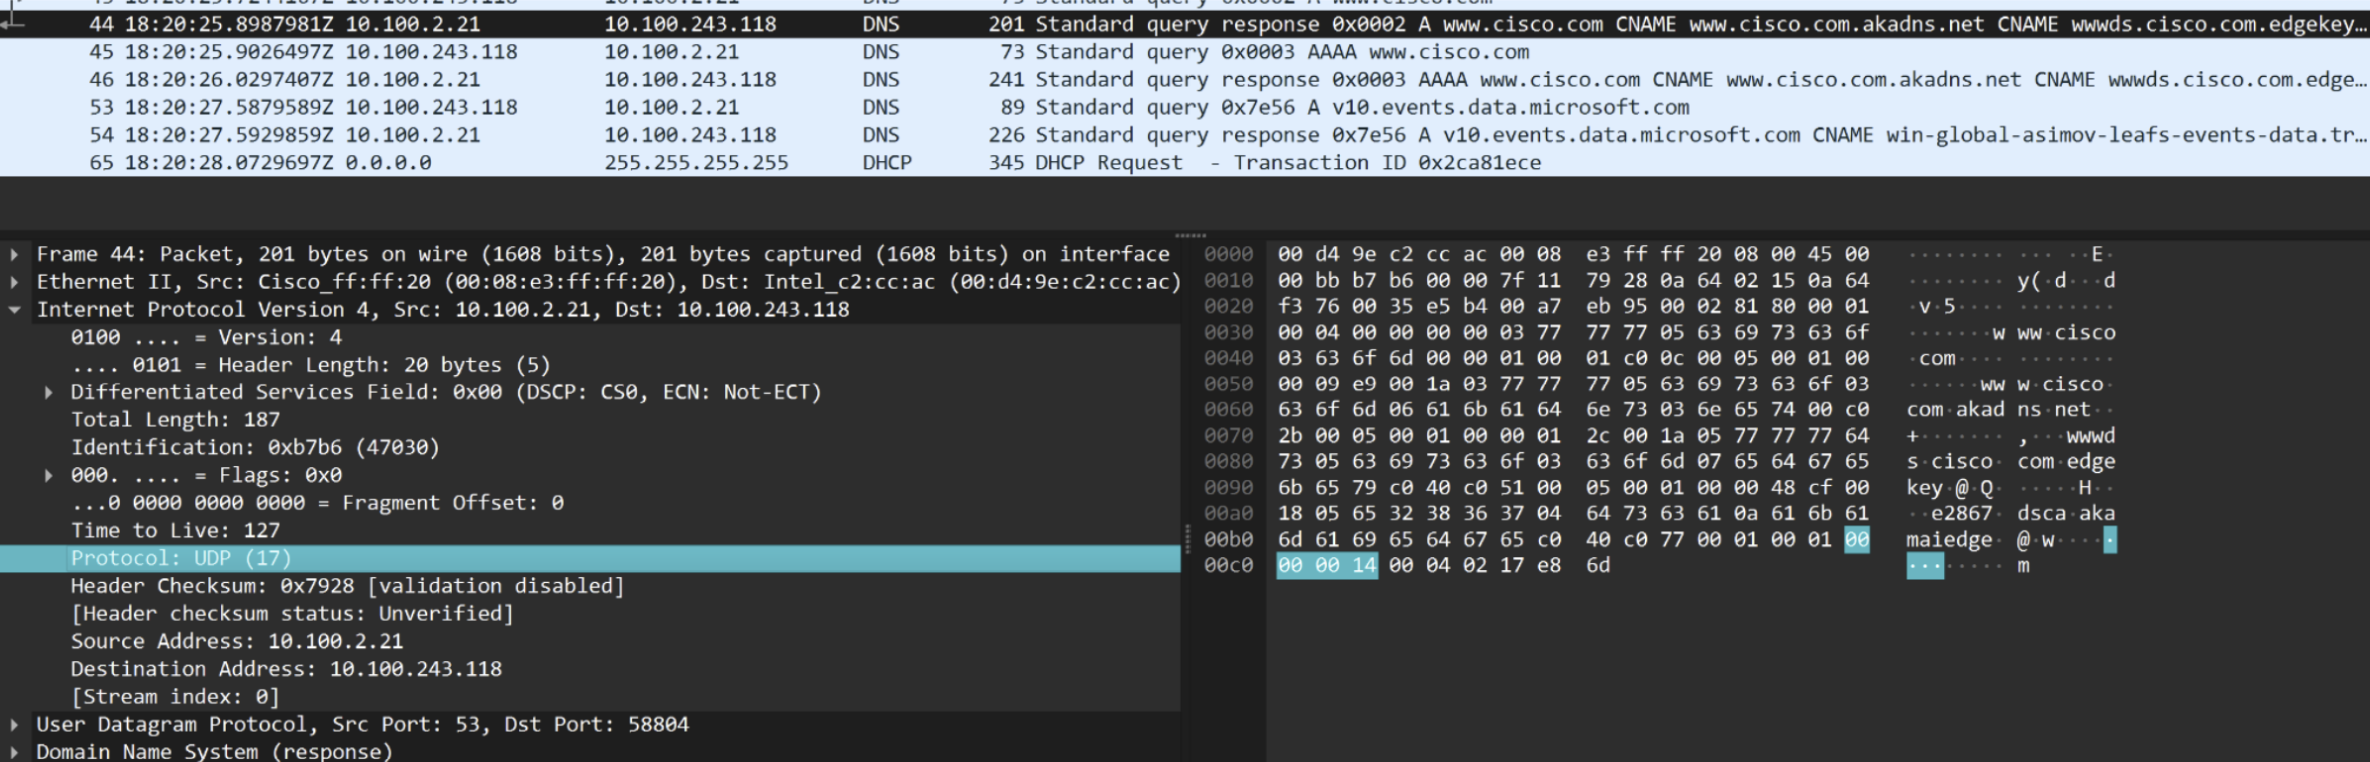
\includegraphics[width=1\linewidth]{imgs/check2_5.png}
    \caption{Valor del campo Protocol en el encabezado IPv4 de un paquete UDP.}
    \label{fig:chk2-5}
\end{figure}


\item \textbf{Examine a pair of UDP packets in which your host sends the first UDP packet and the second UDP packet is a reply to this first UDP packet. Describe the relationship between the port numbers in the two packets.}

En la consulta DNS, nuestro equipo envía el paquete desde puerto 54165 hacia el puerto 53. En la respuesta, los puertos aparecen invertidos: 53 es el origen y el mismo puerto 54165 pasa a ser el destino (Fig.~\ref{fig:chk2-7} y (Fig.~\ref{fig:chk2-8}).).



\end{enumerate}












\subsection{Checkpoint3: Python UDP Implementation (Loopback)}

\begin{enumerate}

\begin{figure}[htbp]
    \centering
    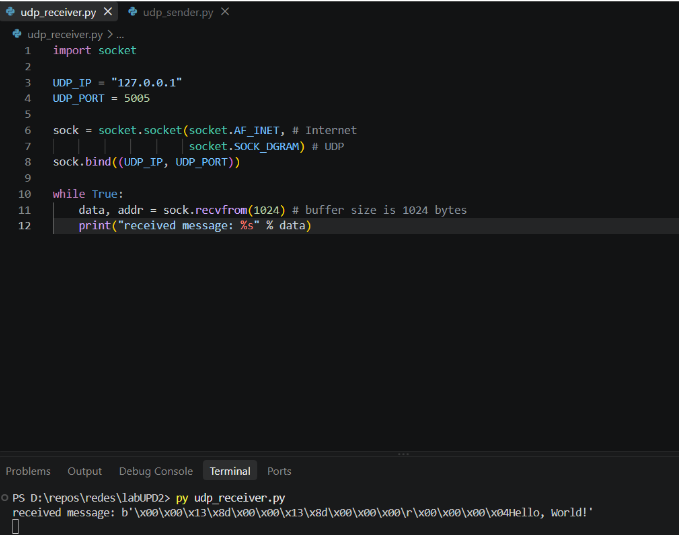
\includegraphics[width=1\linewidth]{imgs/check3_1.png}
    \caption{Código y salida del receptor UDP configurado en 127.0.0.1:5005.}
    \label{fig:chk3-1}
\end{figure}

\begin{figure}[htbp]
    \centering
    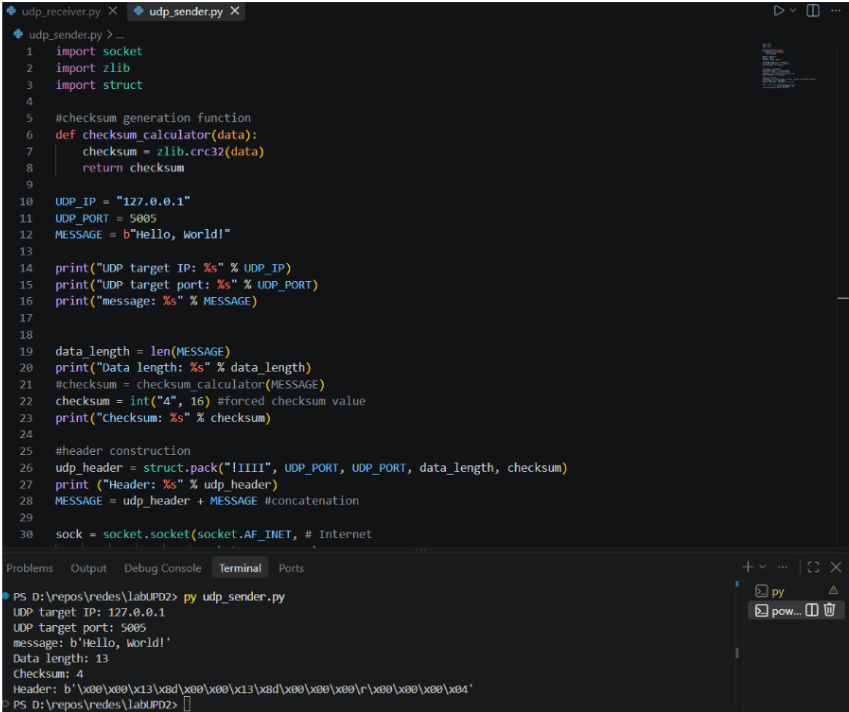
\includegraphics[width=1\linewidth]{imgs/check3_18.png}
    \caption{Código y salida del emisor UDP configurado para enviar al puerto 5005.}
    \label{fig:chk3-18}
\end{figure}


\item \textbf{Does the received header transmitted the data defined in our python program?}

Sí, el header recibido si transmite la data definida por el programa de python. Esto se observa en el mensaje impreso en el sender indica el header 
\begin{lstlisting}[basicstyle=\ttfamily\footnotesize,breaklines=true]
    b'\x00\x00\x13\x8d\x00\x00\x13\x8d\x00\x00\x00\r\x00\x00\x00\x04'
\end{lstlisting}  
es el mismo que se observa en el mensaje que recibió el receiver.(Fig.~\ref{fig:chk3-1})


\item \textbf{What’s the UDP IP on the code.}
La UDP IP definida en el código es 127.0.0.1. (Fig.~\ref{fig:chk3-1})

\item \textbf{Analyze the UDP package and explain the UDP datagram.}

El origen de este datagrama sería el  49825 y lo está enviando al 5005. Cuenta con un tamaño de 37 y el Checksum es 0xc31b [unverified]. El unverified significa que el wireshark no ha aplicado el algoritmo matemático para verificar si es que la data se corrompió o si se pierde información durante el envío. (Fig.~\ref{fig:chk3-2})

\begin{figure}[htbp]
    \centering
    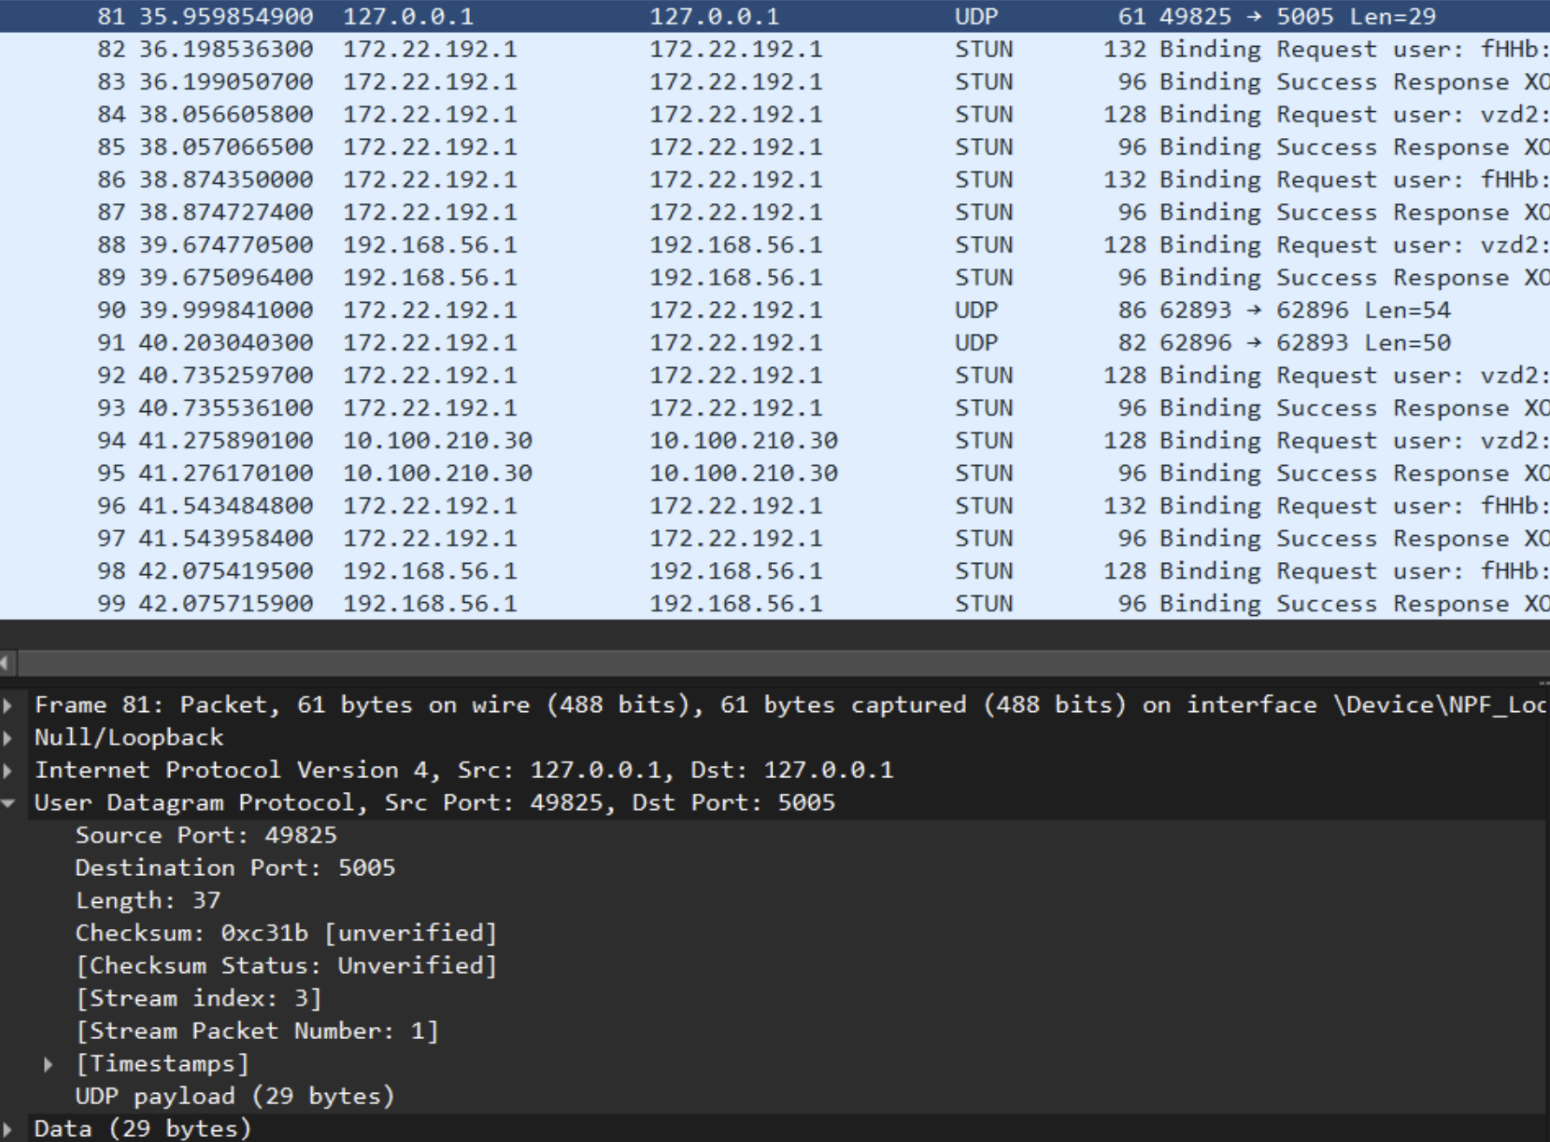
\includegraphics[width=1\linewidth]{imgs/check3_2.png}
    \caption{Datagrama UDP enviado por loopback al puerto 5005.}
    \label{fig:chk3-2}
\end{figure}


\item \textbf{Answer, what would you need to do to send the UDP packet from one computer to a different one? Is any material required? How about the IP configuration?}

Para poder mandar un paquete UDP de una computadora a otra se necesitaría que las computadoras estén conectadas a la misma red para poder asignarles direcciones IP que pertenezcan a la misma subred. No se necesita ningún material adicional. En cuanto a la configuración de la IP, en el código del emisor se debe poner la dirección IP y el puerto UDP del reciever, mientras que el receptor debe tener abierto un puerto UDP para poder escuchar en el puerto que se envía el paquete. 



\item \textbf{Compare the UDP checksum field in at least two captured packets. Was the checksum calculated and validated correctly? Explain how you verified this.}

No, como nos dice que el status del Checksum es unverified, significa que el wireshark decidió no realizar los cálculos para verificar el estado de la información recibida y comprarla con la enviada. La manera en la que se debería verificar es que el emisor aplica un algoritmo matemático en el cuál obtiene un número que se coloca en el header del emisor. Luego al recibir la información el receptor, vuelve a ejecutar el mismo algoritmo para ver si el número que obtiene tras el algoritmo coincide con el mismo que obtuvo el emisor. Si los números no coinciden, significa que la información se corrompe o se perdió parte de esta. (Fig.~\ref{fig:chk3-3} y Fig.~\ref{fig:chk3-16})

\begin{figure}[htbp]
    \centering
    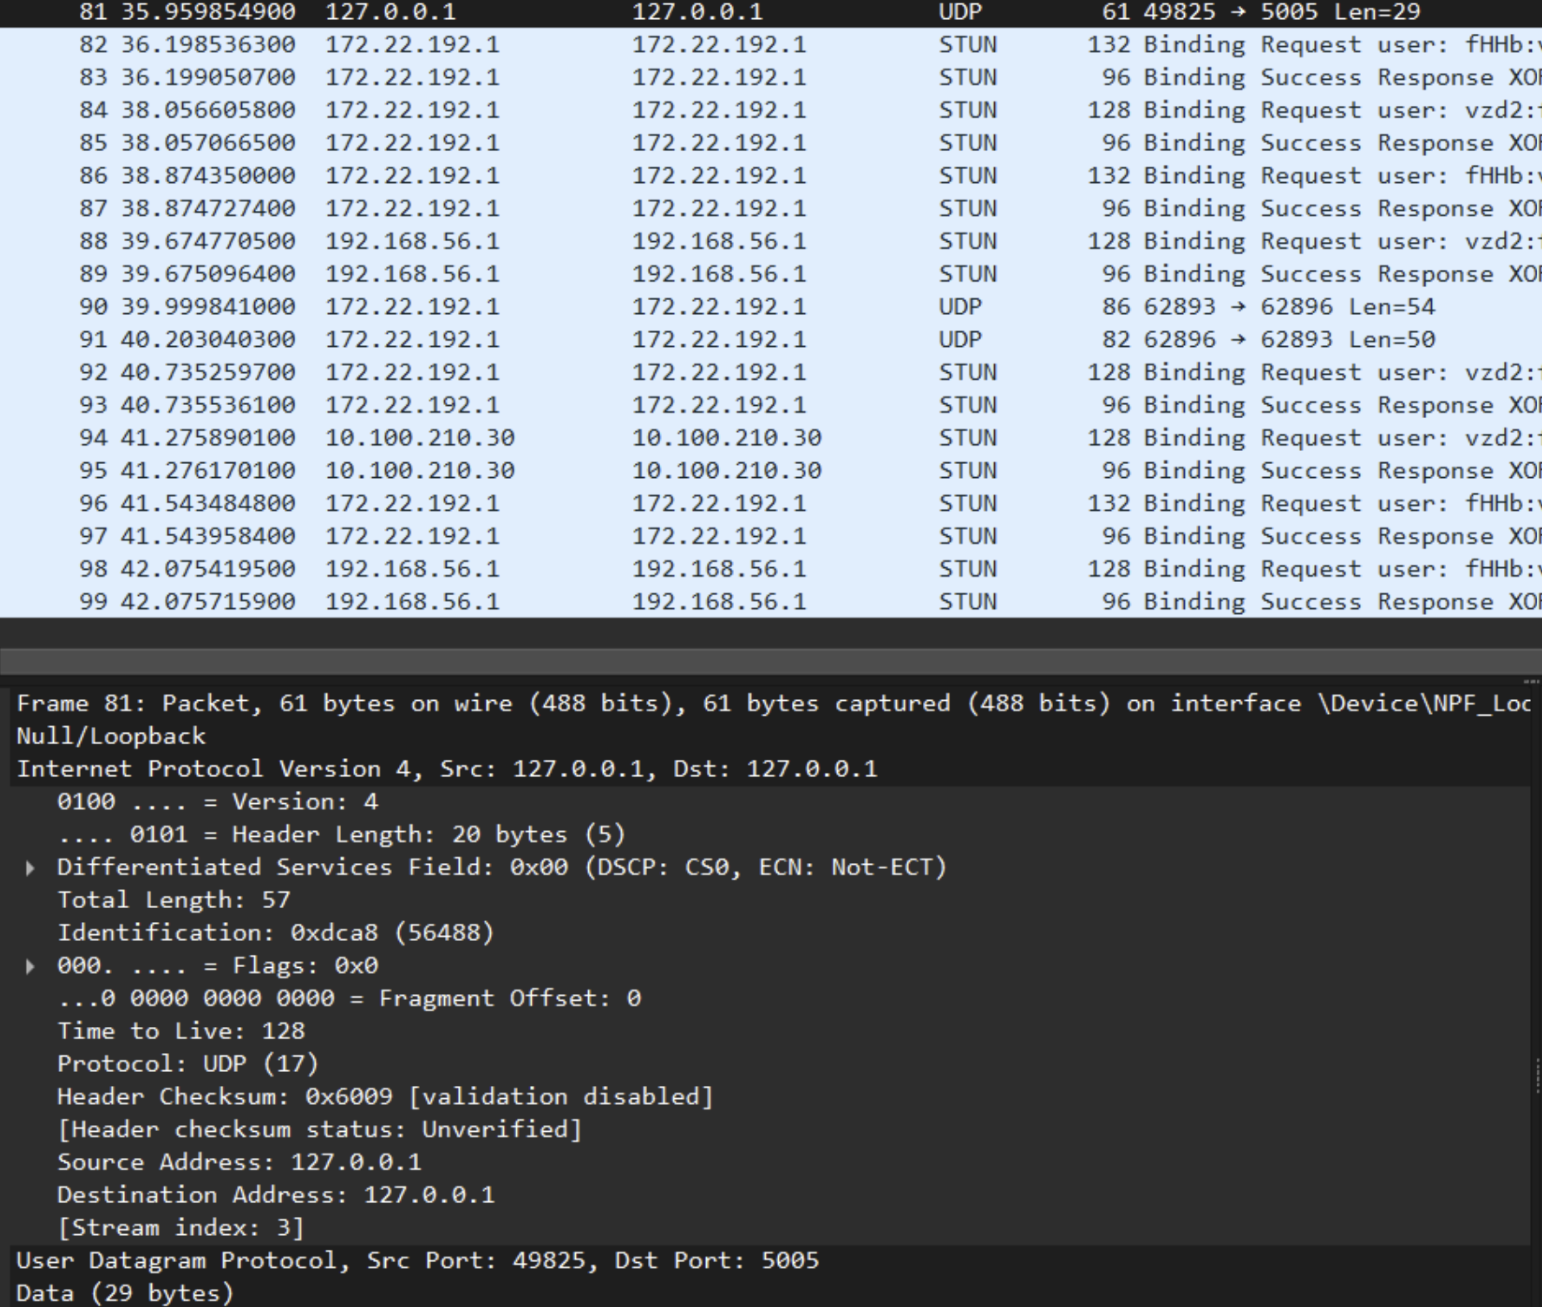
\includegraphics[width=1\linewidth]{imgs/check3_3.png}
    \caption{Encabezado IPv4 del datagrama local, incluido su valor TTL.}
    \label{fig:chk3-3}
\end{figure}

\begin{figure}[htbp]
    \centering
    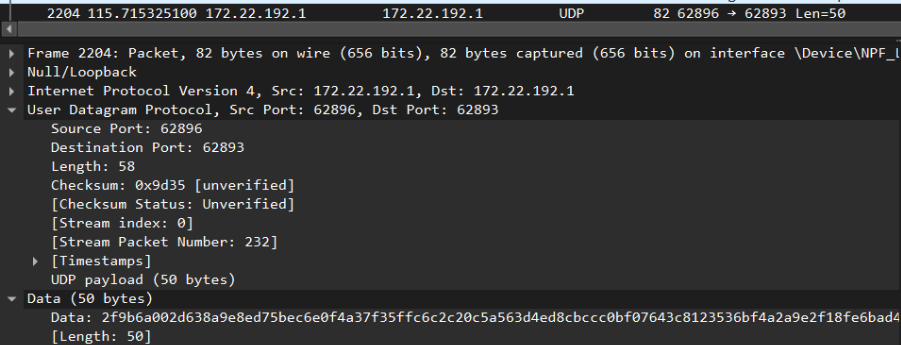
\includegraphics[width=1\linewidth]{imgs/check3_16.png}
    \caption{Campos del datagrama UDP enviado mediante loopback.}
    \label{fig:chk3-16}
\end{figure}


\item \textbf{Examine the Time to Live (TTL) field in the IP header of the UDP packet. Why is the TTL value what it is, and how would it change in a multi-hop real network scenario?}

El ttl obtenido en este paquete es el 128. Este es el valor predeterminado que tiene Windows cuando un paquete IP se crea. Este valor se ha mantenido debido a que la direccion de origen y destino son las mismas, asi que al no haber viajado a un router externo, el valor se mantiene como el mismo. Por cada salto que realizaría en un escenario real en la web el TTL se reduce en 1. Si es que este valor llega a 0, la web nos botará el mensaje de Time limit Exceeded y el router descarta el paquete. (Fig.~\ref{fig:chk3-17})

\begin{figure}[htbp]
    \centering
    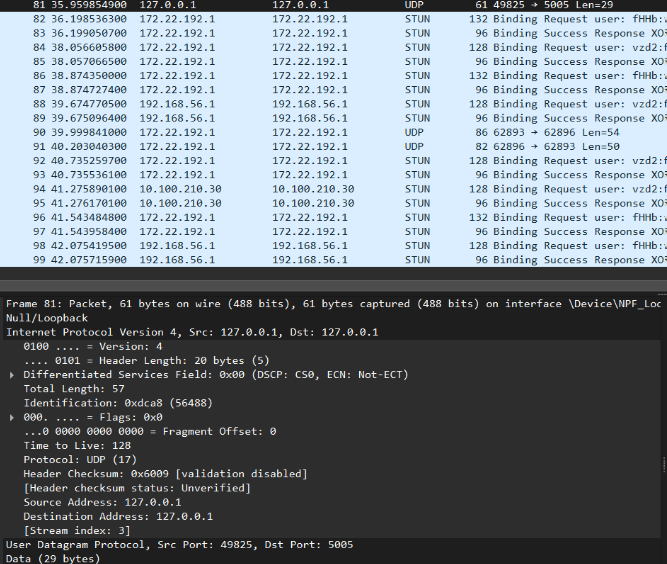
\includegraphics[width=1\linewidth]{imgs/check3_17.png}
    \caption{Encabezado IPv4 del paquete UDP capturado en la interfaz de loopback.}
    \label{fig:chk3-17}
\end{figure}


\item \textbf{Explore how Wireshark differentiates between application-layer protocols when using UDP (e.g., DNS, DHCP). Is your custom message interpreted as a known protocol? Why or why not?}

Wireshark revisa cuales son los puerto de origen y destino y verifica con cual coincide (53 para DNS, 67/68 DHCP). Si el puerto es desconocido, wireshark inspecciona en los primeros bytes patrones que se pueden encontrar en ciertos protocolos. Ahora mismo nuestro mensaje no lo esta aceptando como un puerto conocido porque el puerto 5005 no es un puerto estandar, ahora mismo lo esta tomando como si fuera data en formato hexadecimal o texto.

\item \textbf{Change the destination IP in the sender script to a non-routable or invalid IP (e.g., 192.0.2.1) and rerun the test. What happens in the capture, and why is there a
difference?}

Al estar intentando enviar a una direccion invalida, no lo va a encontrar en el loop, asi que por eso tratara de encontrarlo en Wi-Fi y así fue. (Fig.~\ref{fig:chk3-4}, Fig.~\ref{fig:chk3-5}, Fig.~\ref{fig:chk3-6})

\begin{figure}[htbp]
    \centering
    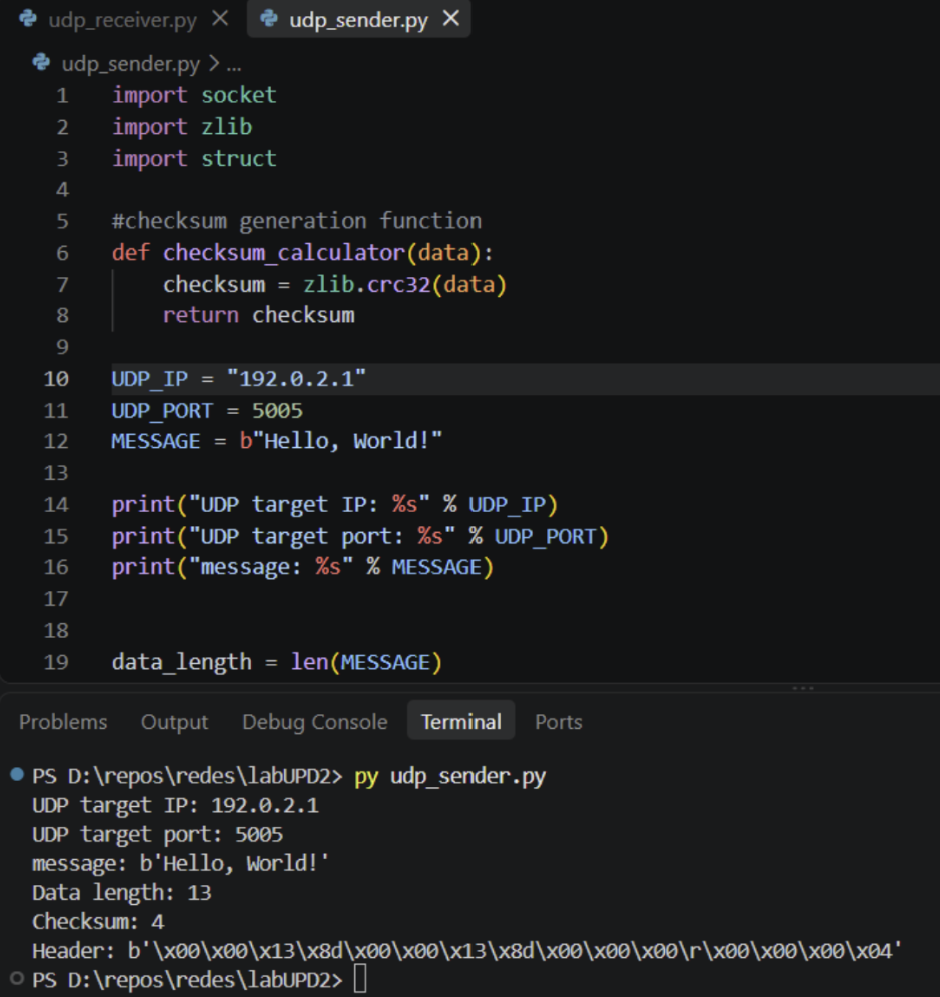
\includegraphics[width=1\linewidth]{imgs/check3_4.png}
    \caption{Código del emisor UDP tras modificar la dirección IP de destino.}
    \label{fig:chk3-4}
\end{figure}

\begin{figure}[htbp]
    \centering
    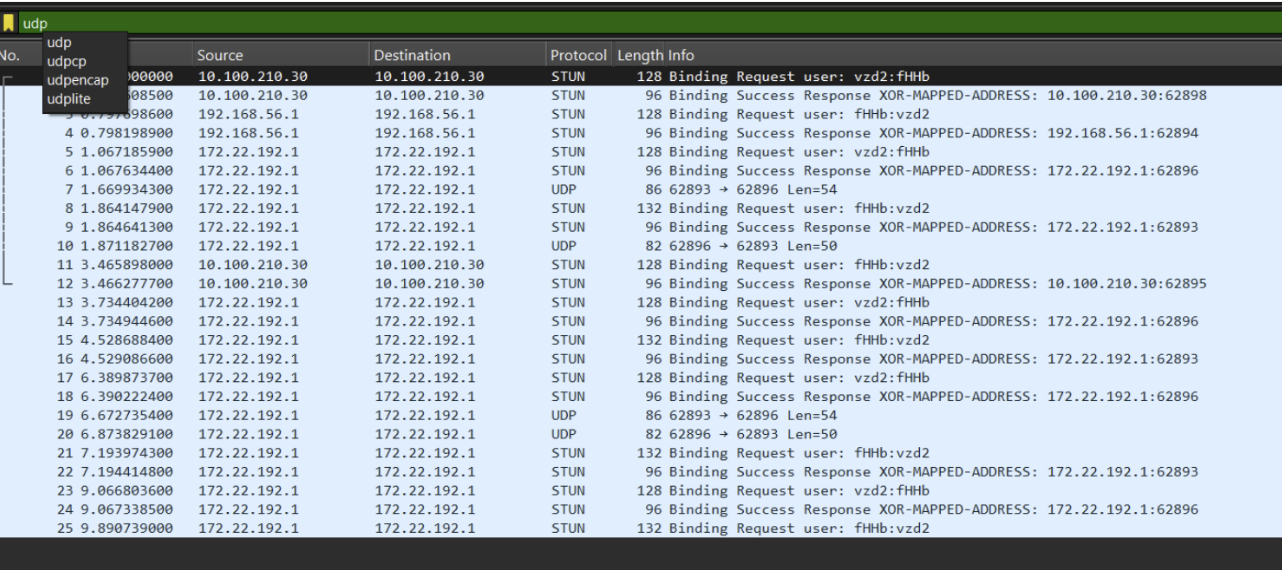
\includegraphics[width=1\linewidth]{imgs/check3_5.png}
    \caption{Salida del emisor UDP después de cambiar la dirección de destino.}
    \label{fig:chk3-5}
\end{figure}

\begin{figure}[htbp]
    \centering
    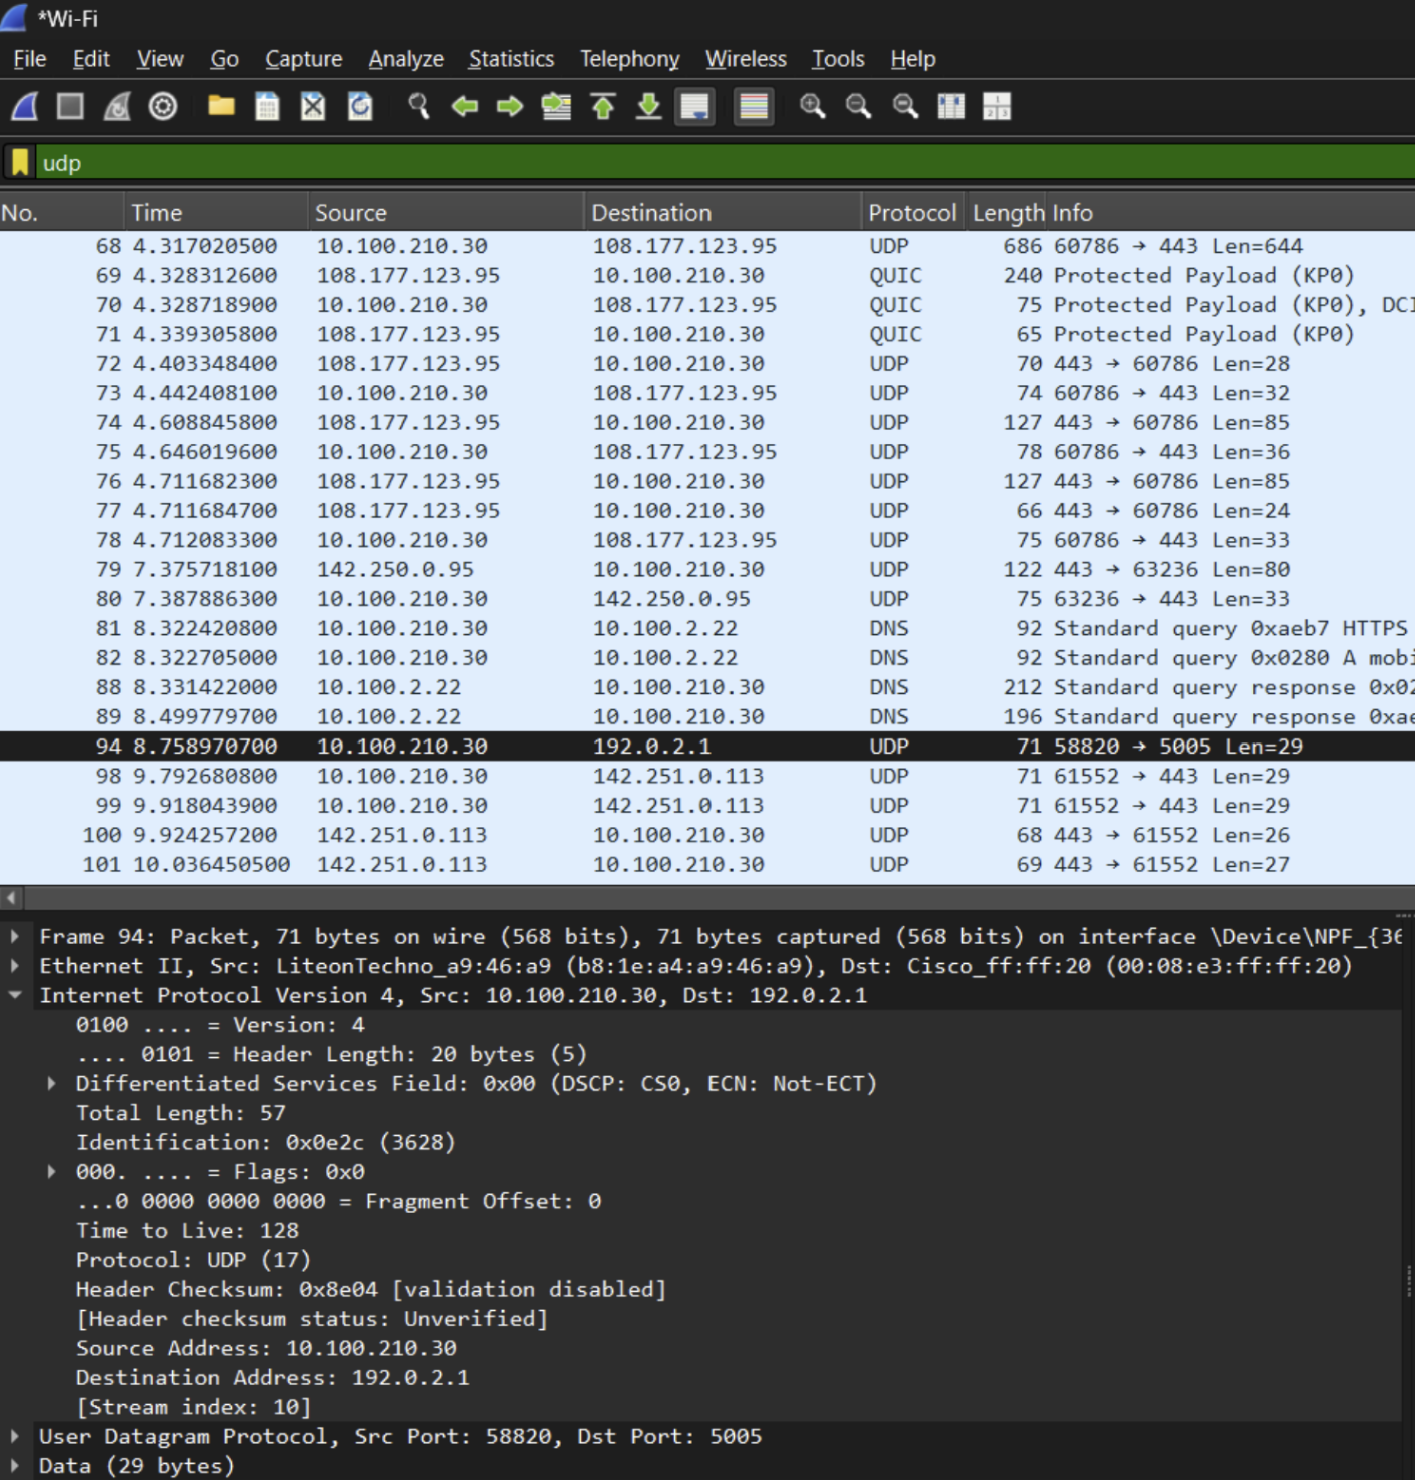
\includegraphics[width=1\linewidth]{imgs/check3_6.png}
    \caption{Datagrama UDP observado tras cambiar el destino fuera de loopback.}
    \label{fig:chk3-6}
\end{figure}

\end{enumerate}


\subsection{Checkpoint 4: Python UDP Implementation (P2P)}


Permitiendo el trafico por puerto UDP 5005  (Fig.~\ref{fig:chk3-7}).

\begin{figure}[htbp]
    \centering
    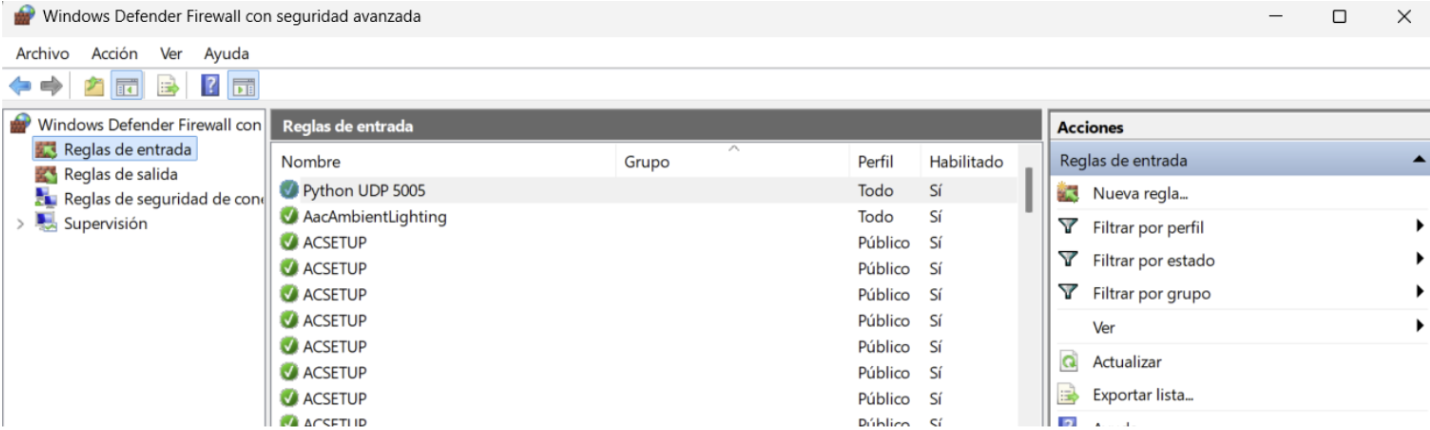
\includegraphics[width=1\linewidth]{imgs/check3_7.png}
    \caption{Regla del firewall que permite el tráfico entrante por el puerto UDP 5005.}
    \label{fig:chk3-7}
\end{figure}

\begin{enumerate}

\item \textbf{Capture the traffic using wireshark.}

\item \textbf{Show the IP addresses of both laptops used.}
\begin{itemize}
    \item Laptop A receptora: (Fig.~\ref{fig:chk3-8}).
    \begin{figure}[htbp]
        \centering
        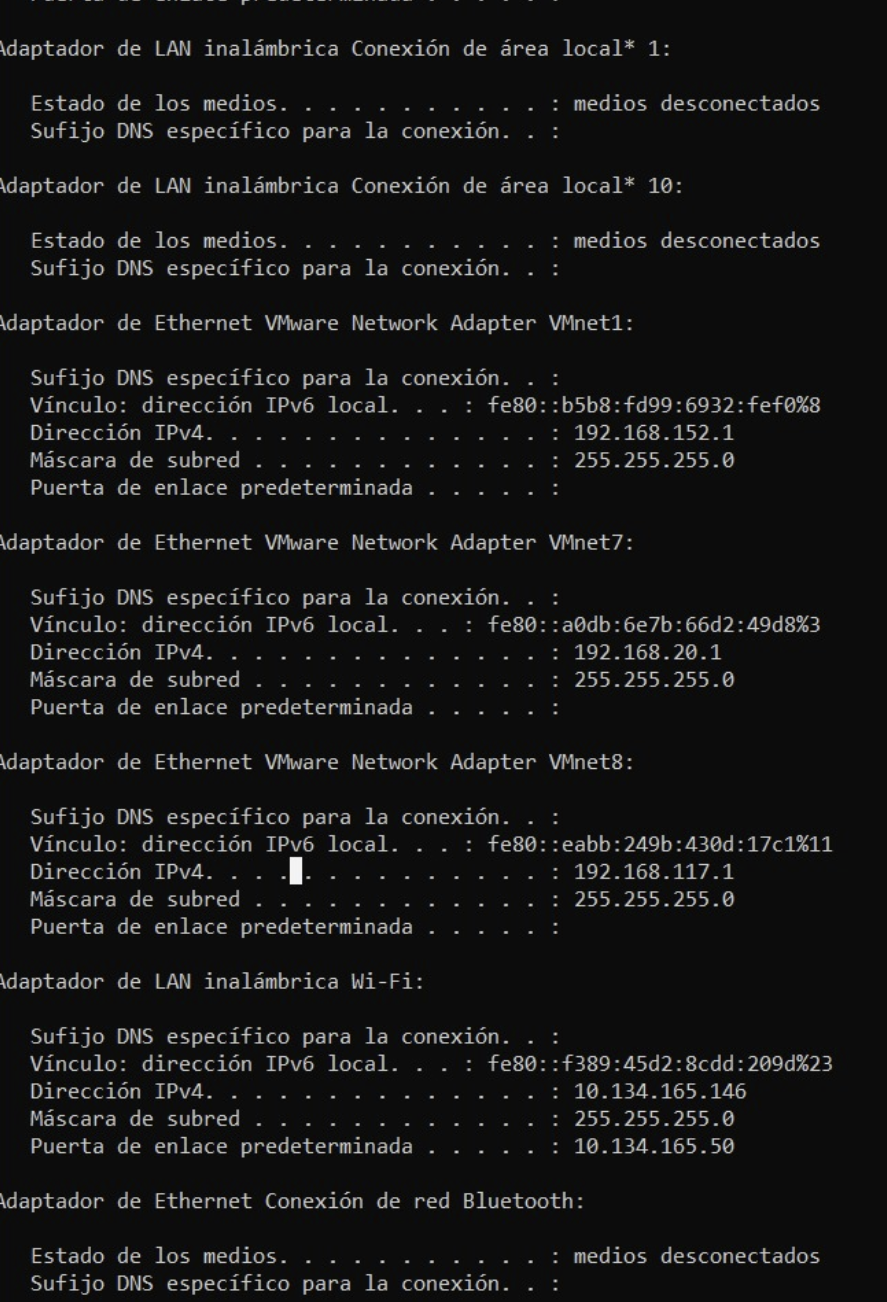
\includegraphics[width=1\linewidth]{imgs/check3_8.png}
        \caption{Configuración IP de la laptop utilizada como receptora.}
        \label{fig:chk3-8}
    \end{figure}

    \item Laptop B emisora: (Fig.~\ref{fig:chk3-9}).
    \begin{figure}[htbp]
        \centering
        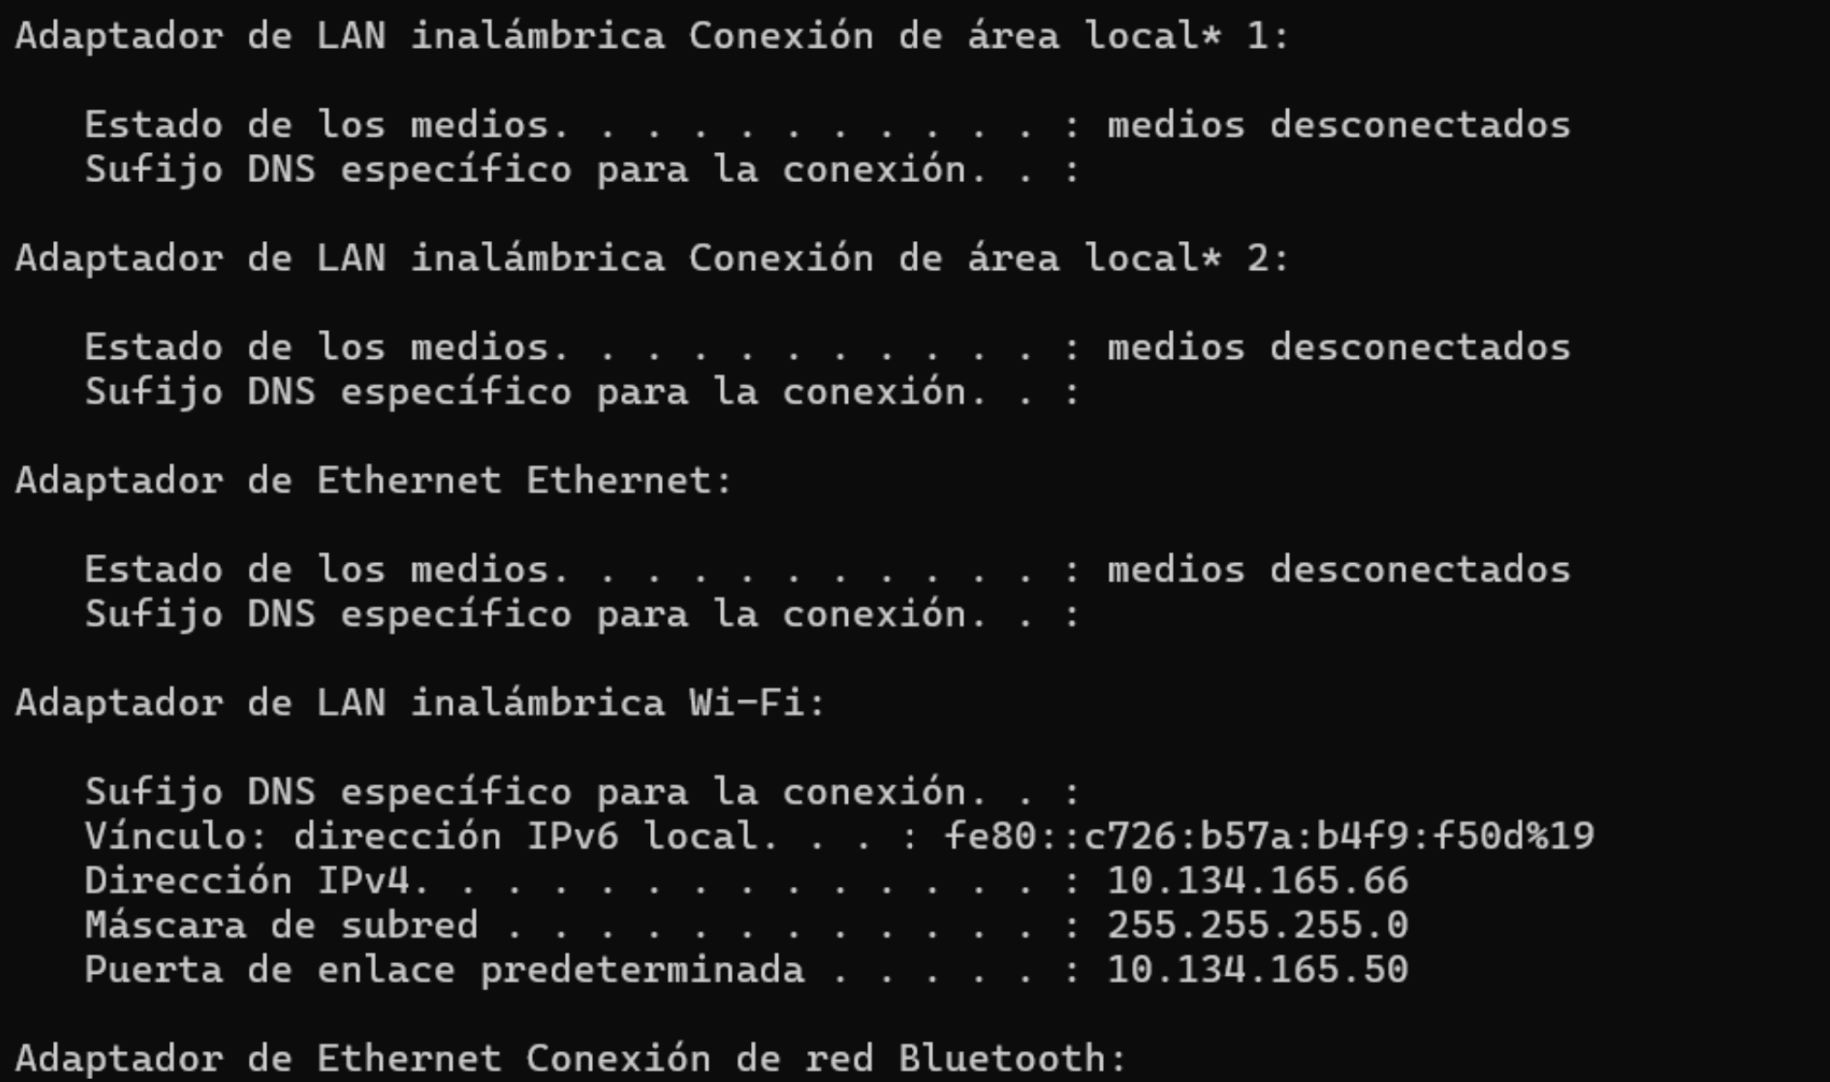
\includegraphics[width=1\linewidth]{imgs/check3_9.png}
        \caption{Configuración IP de la laptop utilizada como emisora.}
        \label{fig:chk3-9}
    \end{figure}

\end{itemize}

\item \textbf{Provide evidence of successful message transmission.}


\begin{itemize}
    \item Emisor:  (Fig.~\ref{fig:chk3-10}).
    \begin{figure}[htbp]
        \centering
        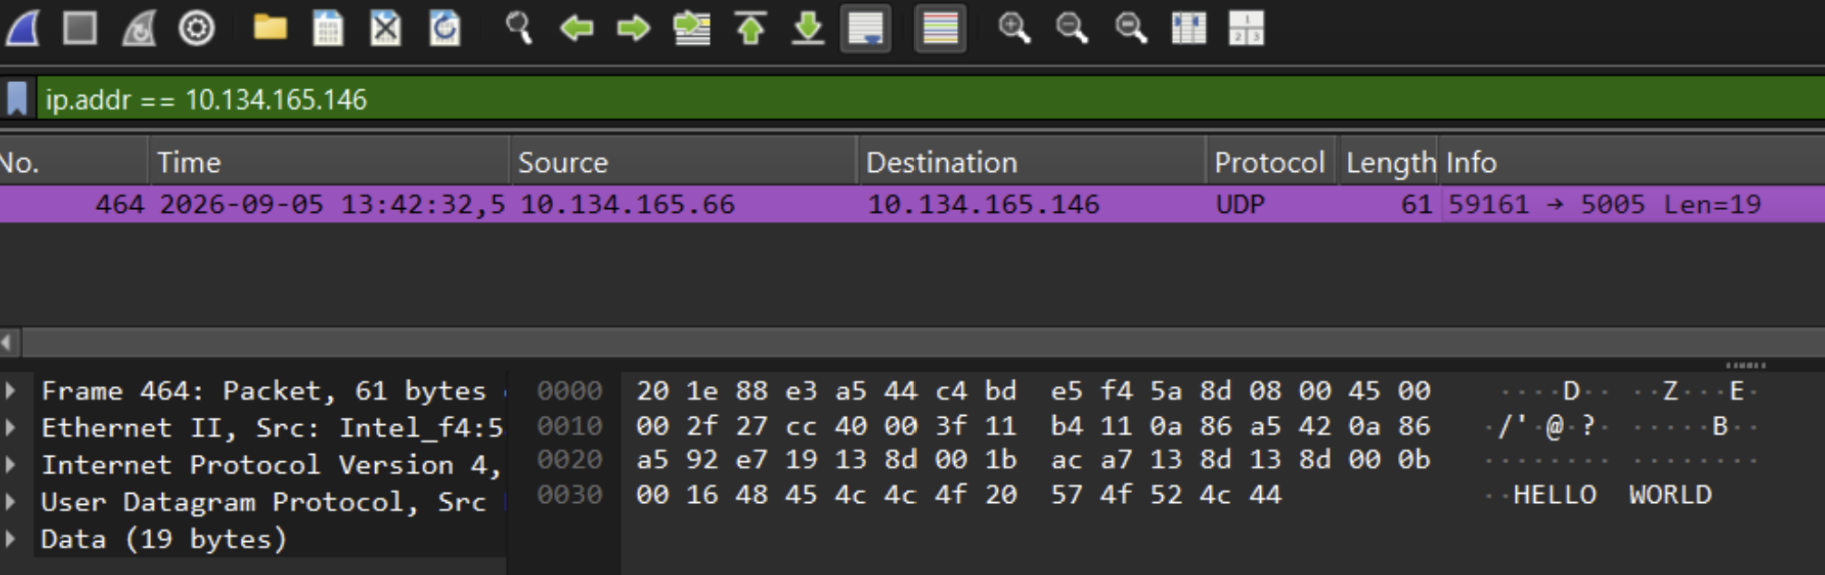
\includegraphics[width=1\linewidth]{imgs/check3_10.png}
        \caption{Datagrama UDP enviado entre las dos laptops por el puerto 5005.}
        \label{fig:chk3-10}
    \end{figure}

    \item Receptor: (Fig.~\ref{fig:chk3-11}).
    \begin{figure}[htbp]
        \centering
        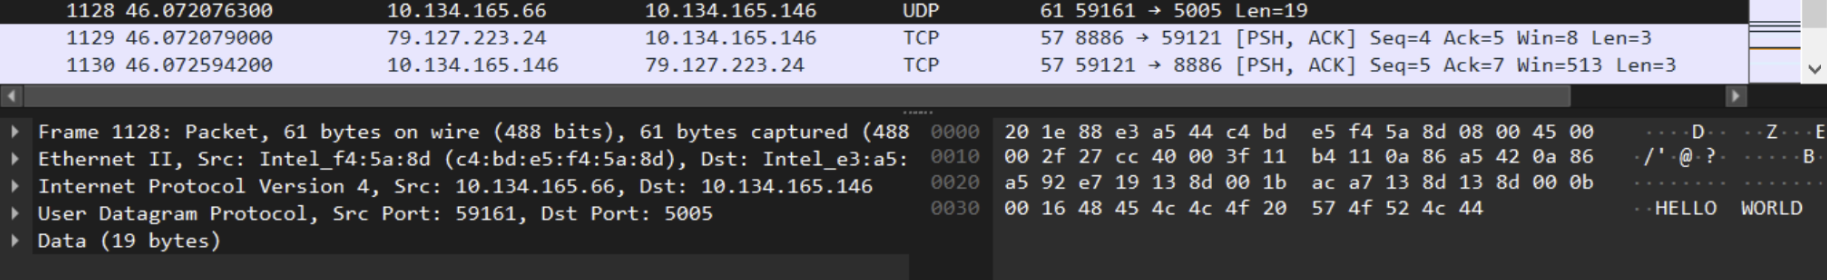
\includegraphics[width=1\linewidth]{imgs/check3_11.png}
        \caption{Paquete capturado durante el intercambio UDP entre las laptops.}
        \label{fig:chk3-11}
    \end{figure}

\end{itemize}


\item \textbf{Describe the message format and how it was handled on the receiver side.}
El mensaje recibido es UDP. Su formato contiene el source port, destination port, length y checksum, seguido del UDP payload, que contiene 19 bytes de datos. (Fig.~\ref{fig:chk3-12}).
\begin{figure}[htbp]
    \centering
    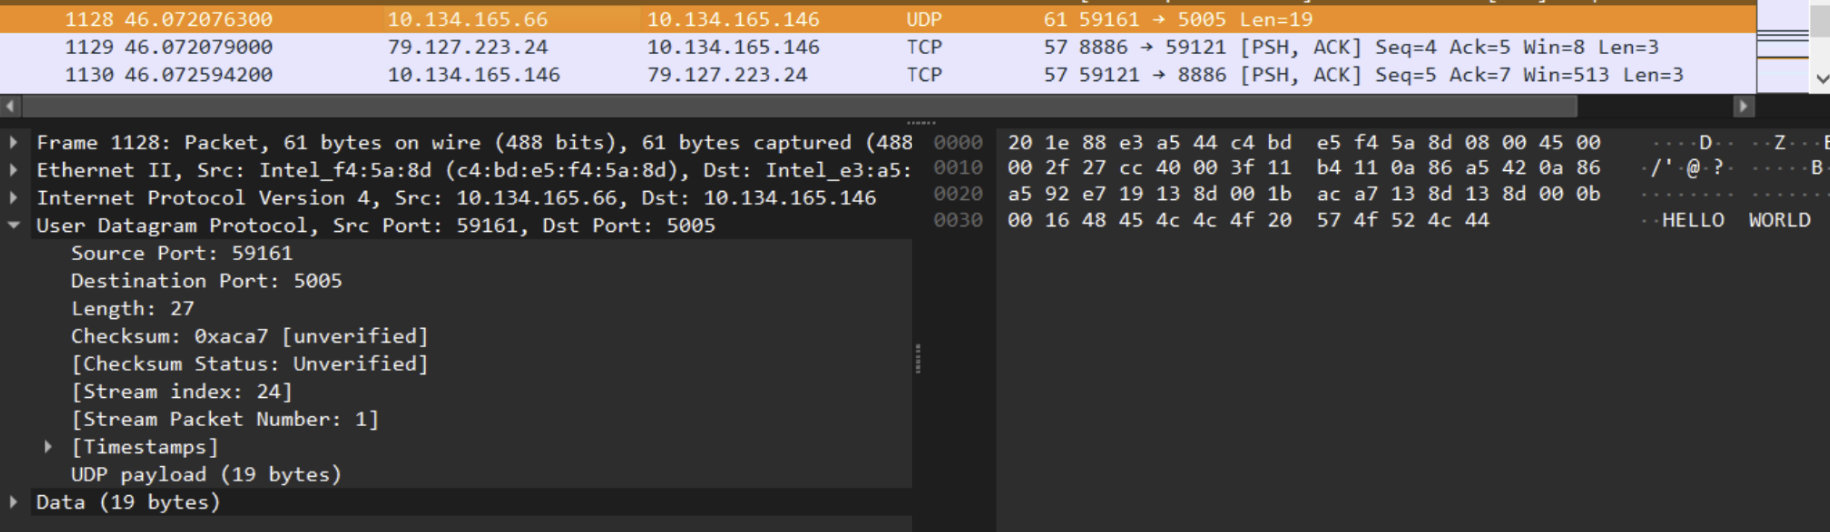
\includegraphics[width=1\linewidth]{imgs/check3_12.png}
    \caption{Puertos, longitud y carga útil del datagrama UDP recibido.}
    \label{fig:chk3-12}
\end{figure}


\item \textbf{Suggest one scenario where UDP would be preferred over TCP and justify.}

UDP puede preferirse en un juego multijugador en tiempo real,
donde los jugadores envían constantemente actualizaciones de
posición y movimiento. También puede ser útil para aplicaciones
interactivas como VoIP o video en vivo. Al no requerir el
\textit{three-way handshake} de TCP ni esperar confirmaciones
propias del protocolo para cada datagrama, UDP permite que la
aplicación priorice las actualizaciones recientes
\cite{rfc768,rfc9293}.

En estos casos, puede ser más útil recibir la siguiente
actualización que recuperar una anterior que ya perdió
relevancia. TCP, en cambio, retransmite los datos perdidos y
los entrega en orden. Si falta un segmento, los datos
posteriores de esa conexión pueden quedar pendientes de
entrega a la aplicación hasta que se recupere, lo que puede
introducir pausas perceptibles \cite{rfc9293,rfc9317}.

\item \textbf{Change the message content and observe how the packet length changes in Wireshark.}

El tamaño del mensaje cambia de 27 a 113. (Fig.~\ref{fig:chk3-13}).
\begin{figure}[htbp]
    \centering
    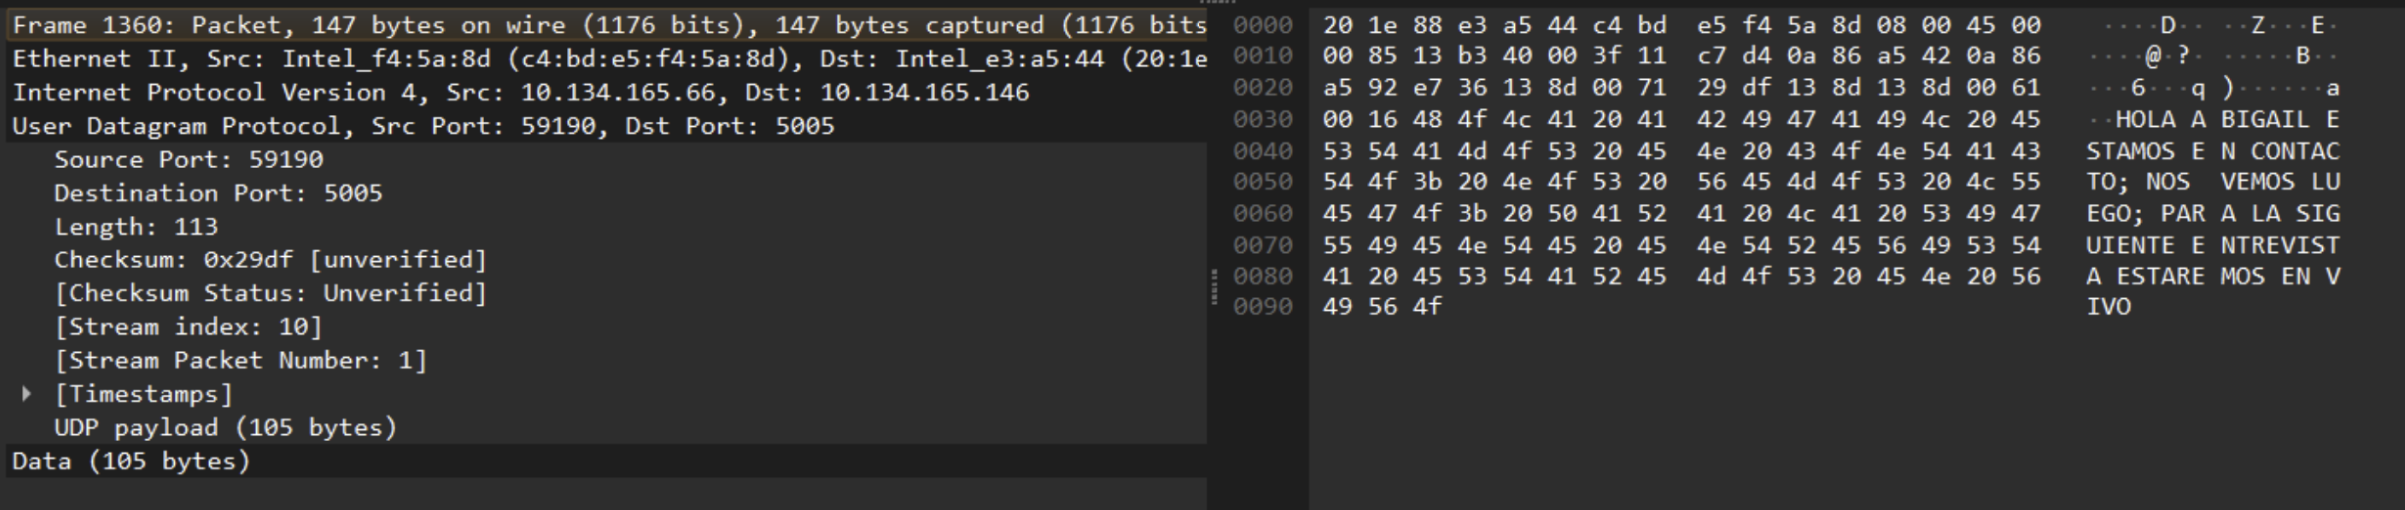
\includegraphics[width=1\linewidth]{imgs/check3_13.png}
    \caption{Datagrama capturado después de modificar el contenido del mensaje.}
    \label{fig:chk3-13}
\end{figure}


\item \textbf{Change the message content specifically to an absurd size (like 12 000 bytes) and see the behaviour of the messages. Is it possible to send messages with that payload size?}

El mensaje es enviado pero no es recibido en el receptor. (Fig.~\ref{fig:chk3-14}).
\begin{figure}[htbp]
    \centering
    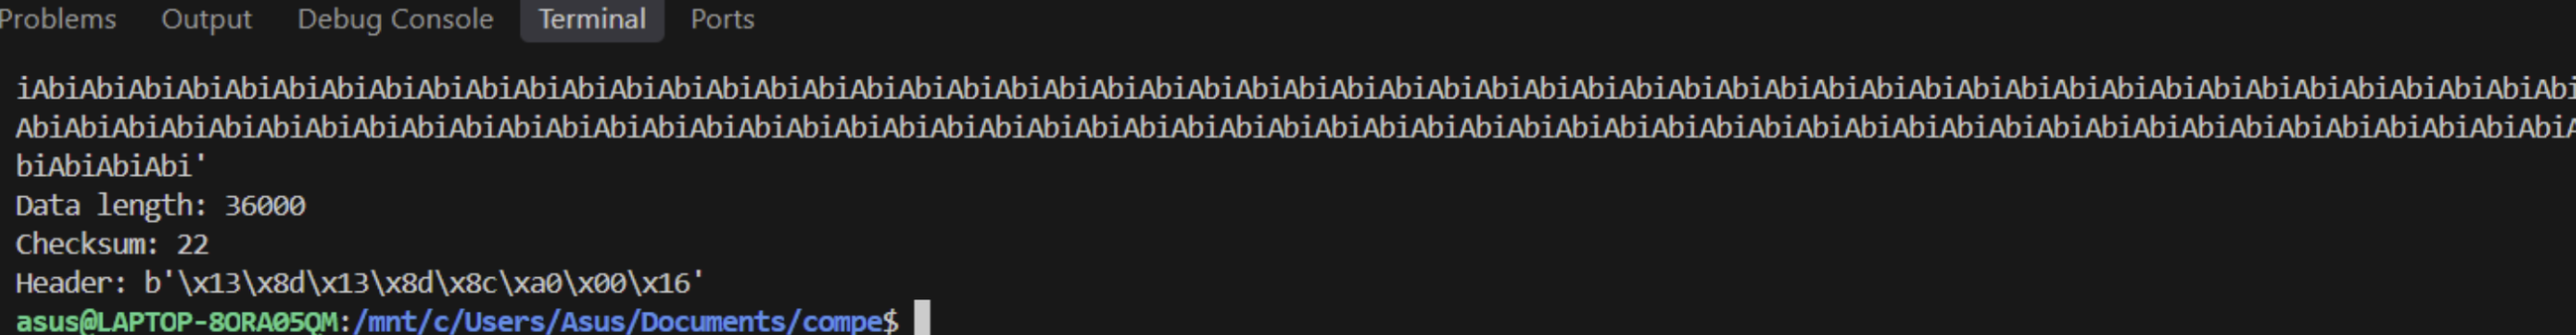
\includegraphics[width=1\linewidth]{imgs/check3_14.png}
    \caption{Salida del programa al intentar enviar un mensaje UDP de gran tamaño.}
    \label{fig:chk3-14}
\end{figure}

El receptor no muestra señales de recibir el mensaje, tampoco se muestra en wireshar. Como máximo se logró recibir un mensaje de 1464 bytes. (Fig.~\ref{fig:chk3-14}).
\begin{figure}[htbp]
    \centering
    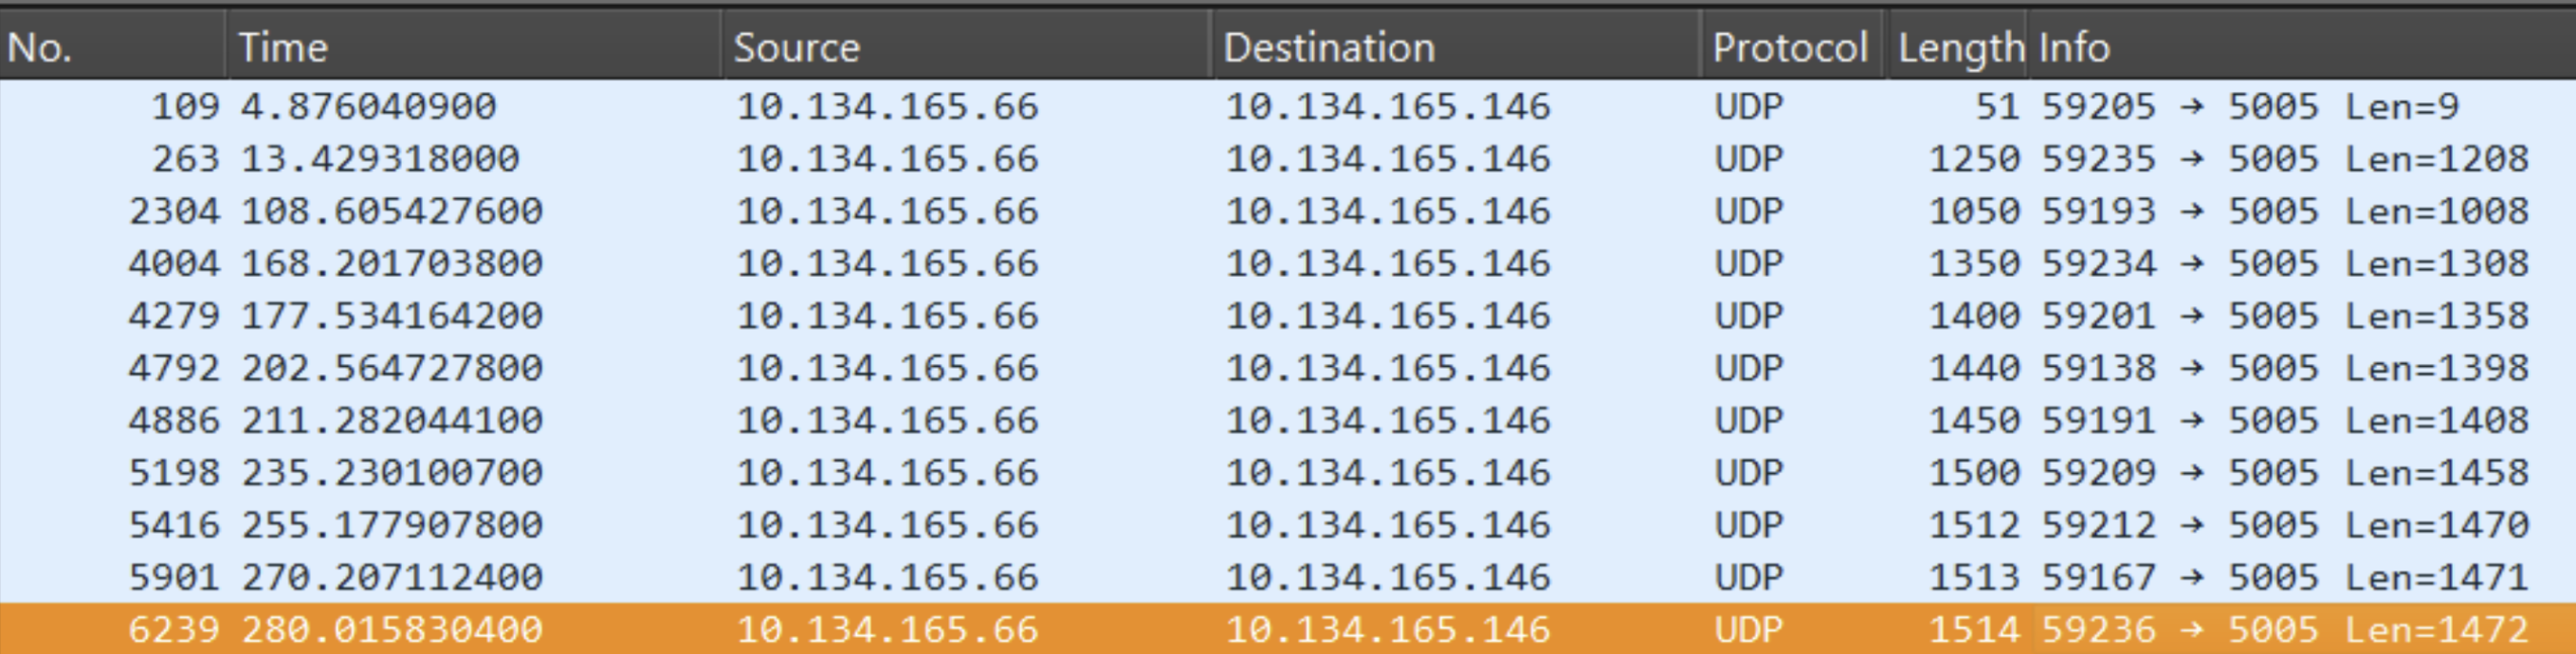
\includegraphics[width=1\linewidth]{imgs/check3_15.png}
    \caption{Longitudes de los datagramas observados durante la prueba con mensajes de distintos tamaños.}
    \label{fig:chk3-15}
\end{figure}

\end{enumerate}




\subsection{Checkpoint 5}

\begin{enumerate}

\item \textbf{ }
\item \textbf{ }
\item \textbf{ }
\item \textbf{ }
\item \textbf{ }
\item \textbf{ }

\end{enumerate}

\subsection{Checkpoint 6}

\begin{enumerate}

\item \textbf{ }
\item \textbf{ }
\item \textbf{ }
\item \textbf{ }
\item \textbf{ }
\item \textbf{ }

\end{enumerate}

\subsection{Checkpoint 7}

\begin{enumerate}

\item \textbf{ }
\item \textbf{ }
\item \textbf{ }
\item \textbf{ }
\item \textbf{ }
\item \textbf{ }

\end{enumerate}

\subsection{Checkpoint 8}

\begin{enumerate}

\item \textbf{ }
\item \textbf{ }
\item \textbf{ }
\item \textbf{ }
\item \textbf{ }
\item \textbf{ }

\end{enumerate}

\subsection{Checkpoint 9: UDP Vulnerabilities: Simulating a Local DDoS (UDP Flood)}

\begin{enumerate}

\item \textbf{On the Victim's Wireshark, go to Statistics > I/O Graphs. Provide a screenshot of the graph showing the sudden spike in packets/bytes per second during the 15-second attack window.}
\begin{itemize}
    \item Atacantes: Fig.~\ref{fig:chk9-1}.
    \begin{figure}[htbp]
        \centering
        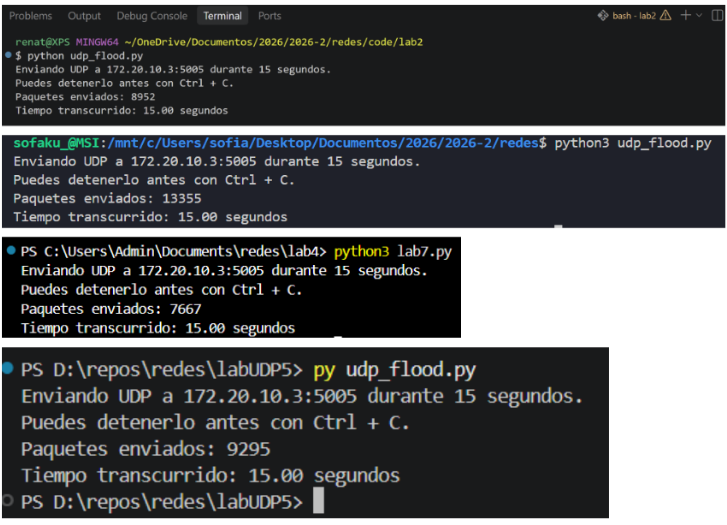
\includegraphics[width=1\linewidth]{imgs/check9-1.png}
        \caption{}
        \label{fig:chk9-1}
    \end{figure}
    \item Victima:  Fig.~\ref{fig:chk9-2}.
    \begin{figure}[htbp]
        \centering
        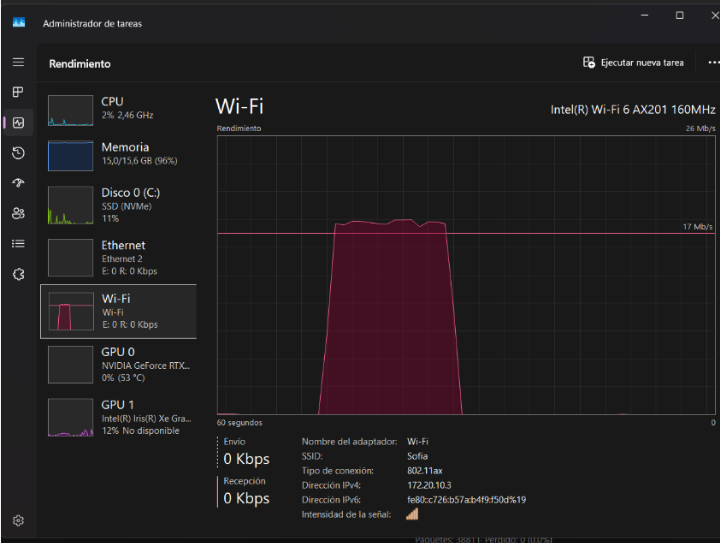
\includegraphics[width=1\linewidth]{imgs/check9-2.png}
        \caption{}
        \label{fig:chk9-2}
    \end{figure}
\end{itemize}


\item \textbf{Based on the Victim's OS Resource Monitor, did you notice a significant spike in Network bandwidth usage or CPU utilization? Explain why an enterprise server might crash if thousands of external computers did this simultaneously.}

Sí, durante la prueba se observó un aumento en el tráfico de red, que alcanzó aproximadamente 18 Mb/s durante el ataque. No se observó un incremento significativo de CPU ya que se observa un uso del 2\% casi constante (Fig.~\ref{fig:chk9-2}). Si miles de computadoras enviaran paquetes simultáneamente a un servidor empresarial, podrían saturar su ancho de banda y agotar sus recursos de procesamiento. Esto podría causar lentitud, pérdida de paquetes y que el servidor dejara de responder a los usuarios legítimos, aunque no necesariamente se apagara. 


\item \textbf{Why is a "Flood" attack fundamentally easier to execute using UDP rather than TCP? (Hint: Think about what TCP requires before sending data, and what UDP ignores).}

Flood attack es fundamentalmente más fácil de ejecutar usando UPD porque UDP no hace handshake antes de enviar datos. Esto permite enviar muchos paquetes seguidos sin esperar una respuesta del receptor. En cambio, TCP requiere establecer una conexión para transferir datos y cuenta con mecanismos de control de flujo y congestión que regulan el envío. 


\item \textbf{One common tactic in real-world UDP attacks is "IP Spoofing," where the attacker forges the Source IP address. Why is it relatively easy to spoof an IP address in a UDP packet, but extremely difficult to do so in a TCP connection?}

Esto se debe principalmente a la seguridad entre ambos. UDP ha sido diseñado con los criterios de simplicidad y velocidad, por eso no cuenta con handshake ni con verificación. Por otra parte, el TCP ha sido designado con un enfoque de seguridad. Este a comparación del protocolo UDP, cuenta con three-way-handshake (SYN, SYN-ACK, ACK).

\item \textbf{If you were the network administrator for the Victim machine, look at the captured flood packets. Is there any legitimate pattern you could use to block this traffic using a Firewall rule? How would the firewall differentiate this flood from legitimate UDP traffic (like a DNS response or a Skype call)?}


Sí se puede identificar el patrón anormal por la gran cantidad de paquetes UDP enviados en muy poco tiempo. El firewall podría bloquear o limitar el tráfico cuando una misma IP supera cierta cantidad de paquetes por segundo. También podría considerar el puerto de destino y el tamaño de los paquetes para detectar el tráfico sospechoso. (Fig.~\ref{fig:chk9-3})

\begin{figure}[htbp]
    \centering
    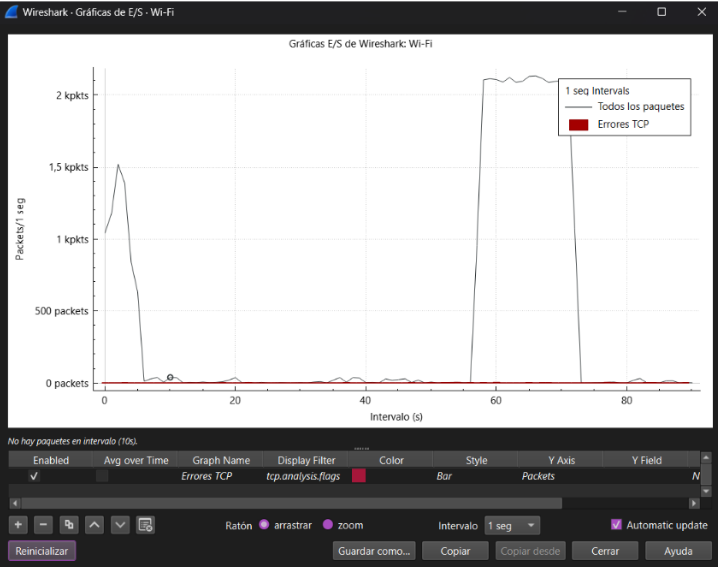
\includegraphics[width=1\linewidth]{imgs/check9-3.png}
    \caption{}
    \label{fig:chk9-3}
\end{figure}


\item \textbf{Research what a "UDP Amplification Attack" is (e.g., DNS or NTP amplification). Briefly explain how an attacker uses a small UDP request to trick a third-party server into sending a massive UDP response to the victim}

\end{enumerate}